% \documentclass[amsmath, amssymb]{revtex4}
% \documentclass[dvips,aoas,preprint]{imsart}
\documentclass[aoas,preprint]{imsart}
% \documentclass{article}
% \input{/Users/joshyv/Research/misc/latex_paper.tex}
%\documentclass[11pt]{article}
\usepackage{a4wide}
\usepackage{apalike}
\usepackage{algorithm}
\usepackage{algpseudocode}
\usepackage{graphicx}% Include figure files
\usepackage{amsmath}
\usepackage{amsfonts}
\usepackage{amsthm}
% \usepackage{charter}
% \usepackage{afterpage}
% \usepackage{cite}
% \usepackage{algorithmic}

%\usepackage{dcolumn}% Align table columns on decimal point
%\usepackage{bm}% bold math
% \RequirePackage[OT1]{fontenc}
% \RequirePackage{amsthm,amsmath,natbib}
%\RequirePackage[colorlinks,citecolor=blue,urlcolor=blue]{hyperref}
% \RequirePackage{hypernat}

\startlocaldefs
\renewcommand{\i}{\backslash i}
\newcommand{\bth}{\mathbf{\theta}}
\newcommand{\w}{w}
\newcommand{\bw}{\mathbf{\w}}
\newcommand{\T}{^{\ensuremath{\mathsf{T}}}}           % transpose
\DeclareMathOperator*{\argmax}{argmax}
\DeclareMathOperator*{\argmin}{argmin}
\newcommand{\bF}{{\bf F}}
\newcommand{\bX}{{\bf X}}
\newcommand{\bn}{{\bf n}}
\newcommand{\bh}{\mathbf{h}}
\newcommand{\hbth}{\widehat{\bth}}
\newcommand{\tbth}{\tilde{\bth}}
\newcommand{\hbw}{\widehat{\bw}}
\newcommand{\sumit}{\sum_{\substack{i \in [1,\ldots,N] \\ t \in [1,\ldots, T]}}}
\long\def\comment#1{}

\endlocaldefs


\begin{document}
	
\begin{frontmatter}
\title{A Bayesian approach for inferring neuronal connectivity from
  calcium fluorescent imaging data}
\runtitle{Inferring neuronal connectivity from calcium imaging}
% \thankstext{T1}{Footnote to the title with the `thankstext' command.}

\begin{aug}
\author{\fnms{Yuriy} \snm{Mishchencko}\thanksref{t1}\ead[label=e1]{yuriy.mishchenko@gmail.com}},
\author{\fnms{Joshua T.} \snm{Vogelstein}\thanksref{t2}\ead[label=e2]{joshuav@jhu.edu}},
\and
\author{\fnms{Liam} \snm{Paninski}\thanksref{t1}
\ead[label=e3]{liam@stat.columbia.edu}
\ead[label=u1,url]{http://www.stat.columbia.edu/$\sim$liam}}

\thankstext{t1}{Department of Statistics and Center for Theoretical Neuroscience, Columbia University}
\thankstext{t2}{Johns Hopkins University}
% \thankstext{t3}{Second supporter of the project}
\runauthor{Y. Mishchenko et al.}

% \affiliation{Some University\thanksmark{m1} and Another University\thanksmark{m2}}

\address{Yuriy Mishchenko\\
Dept. of Statistics and \\
Center for Theoretical Neuroscience\\
Columbia University \\
1255 Amsterdam Ave \\
New York, NY 10027 \\
\printead{e1}\\
% \phantom{E-mail:\ }\printead*{e1}
}

\address{Joshua Vogelstein\\
Johns Hopkins University\\
3400 N. Charles St.\\
Baltimore, MD, 21205 \\
\printead{e2}\\
% \printead{u1}
}

\address{Liam Paninski\\
Dept. of Statistics and \\
Center for Theoretical Neuroscience\\
Columbia University \\
1255 Amsterdam Ave \\
New York, NY 10027 \\
\printead{e3}\\
\printead{u1}}

\end{aug}

\begin{abstract}
Deducing the structure of neural circuits is one of the central
problems of modern neuroscience.  Recently-introduced calcium
fluorescent imaging methods permit experimentalists to observe network
activity in large populations of neurons, but these techniques provide
only indirect observations of neural spike trains, with limited time
resolution and signal quality.  In this work, we present a Bayesian
approach for inferring neural circuitry given this type of imaging
data.  We model the network activity in terms of a collection of
coupled hidden Markov chains, with each chain corresponding to a
single neuron in the network and the coupling between the chains
reflecting the network's connectivity matrix.  We derive a Monte Carlo
Expectation-Maximization algorithm for fitting the model parameters;
to obtain the sufficient statistics in a computationally-efficient
manner, we introduce a specialized blockwise-Gibbs algorithm for
sampling from the joint activity of all observed neurons given the
observed fluorescence data.  We perform large-scale simulations of
randomly connected neuronal networks with biophysically realistic
parameters and find that the proposed methods can accurately infer the
connectivity in these networks given reasonable experimental and
computational constraints.  In addition, the estimation accuracy may
be improved significantly by incorporating prior knowledge about the
sparseness of connectivity in the network, via standard L$_1$
penalization methods.
\end{abstract}

\begin{keyword}[class=AMS]
%\kwd[Primary ]{60K35}
%\kwd{60K35}
%\kwd[; secondary ]{60K35}
\end{keyword}

\begin{keyword}
\kwd{Sequential Monte Carlo}
\kwd{Metropolis-Hastings}
\kwd{Spike train data}
\kwd{Point process}
\kwd{Generalized linear model}
\end{keyword}

\end{frontmatter}
	

\section{Introduction}
\label{intro}
Since Ramon y Cajal discovered that the brain is a rich and dense
network of neurons \cite{RamonyCajal04,RamonyCajal23}, neuroscientists
have been intensely curious about the details of these networks, which
are believed to be the biological substrate for memory, cognition, and
perception. While we have learned a great deal in the last century
about ``macro-circuits'' (the connectivity between coarsely-defined
brain areas), a number of key questions remain open about
``micro-circuit'' structure, i.e., the connectivity within populations
of neurons at a fine-grained cellular level.  Two complementary
strategies for investigating micro-circuits have been pursued
extensively.  \emph{Anatomical} approaches to inferring circuitry do
not rely on observing neural activity; some recent exciting examples
include array tomography \cite{MichevaSmith07}, genetic ``brainbow''
approaches \cite{Brainbow07}, and serial electron microscopy
\cite{Briggman2006}. Our work, on the other hand, takes a
\emph{functional} approach: our aim is to infer micro-circuits by
observing the simultaneous activity of a population of neurons,
without making direct use of fine-grained anatomical measurements.

Experimental tools that enable simultaneous observations of the
activity of many neurons are now widely available. While arrays of
extracellular electrodes have been exploited for this purpose
\cite{HATS98,HARR03,Stein04,Santhanam06,Harris07}, the arrays most
often used \emph{in vivo} are inadequate for inferring monosynaptic
connectivity in very large populations of neurons, as the
inter-electrode spacing is typically too large to record from
neighboring neurons\footnote{It is worth noting, however, that
multielectrode arrays which have been recently developed for use in
the retina are capable of much denser sampling
\cite{Berry2004,Litke2004,Petrusca07,PILL07}.}; importantly,
neighboring neurons are more likely connected to one another than than
distant neurons \cite{Abeles91,Braitenberg1998}.  Alternately,
calcium-sensitive fluorescent indicators allow us to observe the
spiking activity of on the order of $10^3$ neighboring neurons
\cite{Tsien89,ImagingManual,CAR03,OHKI05} within a micro-circuit.
Some organic dyes achieve sufficiently high signal-to-noise ratios
(SNR) that individual action potentials (spikes) may be resolved
\cite{ImagingManual}, and bulk-loading techniques enable
experimentalists to simultaneously fill populations of neurons with
such dyes \cite{StosiekKonnerth03}. In addition, genetically encoded
calcium indicators are under rapid development in a number of groups,
and are approaching SNR levels of nearly single spike accuracy as well
\cite{WallaceHasan08}. Microscopy technologies for collecting
fluorescence signals are also rapidly developing. Cooled CCDs for
wide-field imaging (either epifluorescence or confocal) now achieve a
quantum efficiency of $\approx 90 \%$ with frame rates up to $60$ Hz
or greater, depending on the field of view \cite{Djurisic04}. For in
vivo work, 2-photon laser scanning microscopy can achieve similar
frame rates, using either acoustic-optical deflectors to focus light
at arbitrary locations in three-dimensional space
\cite{Iyer06,SalomeBourdieu06,ReddySaggau08}, or resonant scanners
\cite{NguyenParker01}. Together, these experimental tools can provide
movies of calcium fluorescence transients from large networks of
neurons with adequate SNR, at imaging frequencies of $30$ Hz or
greater, in both \emph{in vitro} and \emph{in vivo} preparations.

Given these experimental advances in functional neural imaging, our
goal is to develop efficient computational and statistical methods to
exploit this data for the analysis of neural connectivity; see Figure
\ref{fig:data_schematic} for a schematic overview.  One major
challenge here is that calcium transients due to action potentials
provide indirect observations, and decay about an order of magnitude
slower than the time course of the underlying neural activity
\cite{ImagingManual,Roxin08}. Thus, to properly analyze the functional
network connectivity, we must incorporate methods for effectively
deconvolving the observed noisy fluorescence signal to obtain
estimates of the underlying spiking rates
\cite{YaksiFriedrich06,GreenbergKerr08,Vogelstein2009}. To this end we
introduce a coupled Markovian state-space model that relates the
observed variables (fluorescence traces from the neurons in the
microscope's field of view) to the hidden variables of interest (the
spike trains and intracellular calcium concentrations of these
neurons), as governed by a set of biophysical parameters including the
network connectivity matrix. Given this model, we derive a Monte Carlo
Expectation Maximization algorithm for obtaining the maximum a
posteriori estimates of the parameters of interest. Standard Monte
Carlo sampling procedures (e.g., Gibbs sampling or sequential Monte
Carlo) are inadequate in this setting, due to the high dimensionality
and non-linear, non-Gaussian dynamics of the hidden variables in our
model; we therefore develop a specialized blockwise-Gibbs approach for
efficiently computing the sufficient statistics.  This strategy
enables us to accurately infer the functional connectivity matrix from
large simulated neural populations, under realistic assumptions about
the dynamics and observation parameters.

\begin{figure}[t!]
	\centering
	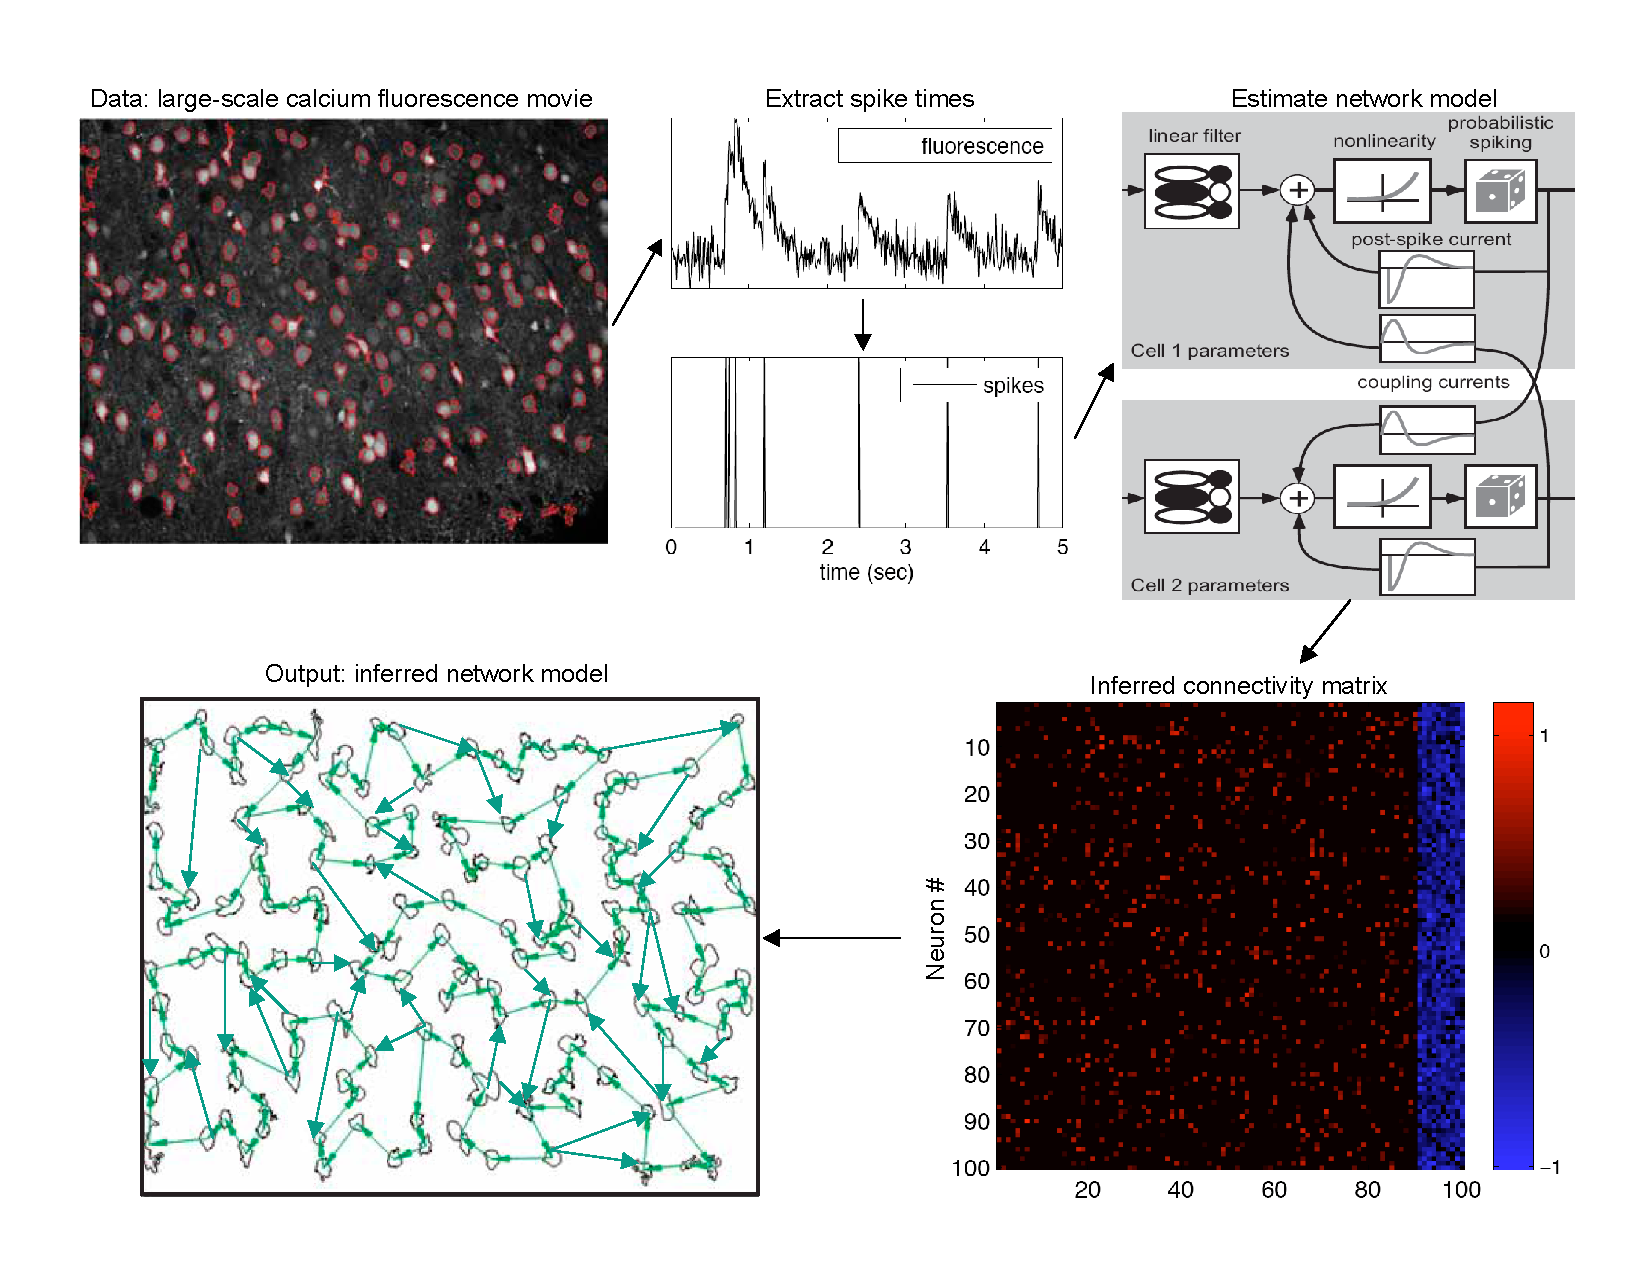
\includegraphics[width=\hsize]{../figs/yuri-paper-schematic}
	\caption{Schematic overview. The raw observed data is a
	large-scale calcium fluorescence movie, which is pre-processed
	to correct for movement artifacts and find
	regions-of-interest, i.e., putative neurons.  (Note that we
	have omitted details of these important preprocessing steps in
	this paper; see, e.g., \cite{CAR03,DombeckTank07} for further
	details.)  Given the fluorescence traces $F_i(t)$ from each
	neuron, we estimate the underlying spike trains (i.e., the
	time series of neural activity) using statistical
	deconvolution methods.  Then we estimate the parameters of a
	network model given the observed data.  Our major goal is to
	obtain an accurate estimate of the network connectivity
	matrix, which summarizes the information we are able to infer
	about the local neuronal microcircuit. This figure adapted
	from personal communications with R.\ Yuste, B.\ Watson, and
	A.\ Packer.}
	\label{fig:data_schematic}
\end{figure}


\section{Methods}
\label{sec:methods}
\subsection{Model}
\label{sec:methods:markov-setup}

We begin by detailing a parametric generative model for the
(unobserved) joint spike trains of all $N$ observable neurons, along
with the observed calcium fluorescence data. Each neuron is modeled as
a generalized linear model (GLM). This class of models is known to
capture the statistical firing properties of individual neurons fairly
accurately
\cite{BRIL88,CSK88,BRIL92,PG00,PAN03d,PAN04c,Rigat06,TRUC05,NYK06,KP06,PILL07,Vidne08,Stevenson2009}. We
denote the $i$-th neuron's activity at time $t$ as $n_i(t)$: in
continuous time, $n_i(t)$ could be modeled as an unmarked point
process, but we will take a discrete-time approach here, with each
$n_i(t)$ taken to be a binary random variable. We model the spiking
probability of neuron $i$ via an instantaneous nonlinear function,
$f(\cdot)$, of the filtered and summed input to that neuron at that
time, $J_i(t)$. This input is composed of: (i) some baseline value,
$b_i$; (ii) some external vector stimulus, $S^{ext}(t)$, that is
linearly filtered by $k_i$; and (iii) spike history terms,
$h_{ij}(t)$, encoding the influence on neuron $i$ from neuron $j$,
weighted by $\w_{ij}$:
\begin{equation} \label{eqn:glm:definition}
\begin{array}{l}
n_i(t) \sim \text{Bernoulli}\left[f\left(J_i(t) \right) \right], \qquad
J_i(t)=b_i+k_i\cdot S^{ext}(t)+\sum \limits_{j=1}^{N} \w_{ij} h_{ij}(t).
\end{array}
\end{equation}

To ensure computational tractability of the parameter inference
problem, we must impose some reasonable constraints on the
instantaneous nonlinearity $f(\cdot)$ (which plays the role of the
inverse of the link function in the standard GLM setting) and on the
dynamics of the spike-history effects $h_{ij}(t)$. First, we restrict
our attention to functions $f(\cdot)$ which ensure the concavity of
the spiking loglikelihood in this model \cite{PAN04c,Escola07}, as we
will discuss at more length below. In this paper, we use
\begin{equation}
f(J) = P\left[n>0 ~|~ n \sim \text{Poiss}\left(e^J\Delta\right)\right] = 1 - \exp[-e^J \Delta]
\end{equation}
(Figure \ref{fig:egfluor}), where the inclusion of $\Delta$, the time step size, ensures that the firing rate scales properly with respect to the time discretization; see \cite{Escola07} for a proof that this $f(\cdot)$ satisfies the required concavity constraints. However, we should note that in our experience the results depend only weakly on the details of $f(\cdot)$ within the class of log-concave models \cite{LD89,PAN04c}.

\begin{figure}[t!]
\centering 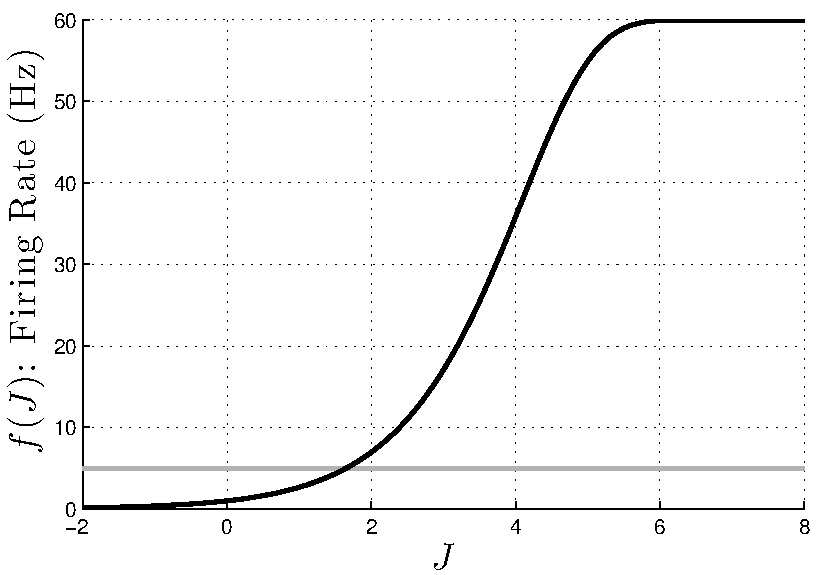
\includegraphics[width=3in]{../figs/fr_vs_J}
\caption{A plot of the firing rate nonlinearity $f(J)$ used in our
  simulations.  Note that the firing
  rate saturates at $1/\Delta$, because of our Bernoulli assumption
  (i.e., the spike count per bin is at most one). Here $\Delta = (60$
  Hz$)^{-1}$.  The horizontal gray line indicates 5 Hz, the baseline
  firing rate for most of the simulations discussed in the Results section.}
\label{fig:egfluor}
\end{figure}

Second, because the algorithms we develop below assume Markovian
dynamics, we model the spike history terms as an autoregressive
process driven by the spike train $n_j(t)$:
\begin{equation} \label{eqn:h:definition}
h_{ij}(t) = (1- \Delta/\tau^h_{ij}) h_{ij}(t- \Delta) +n_j(t-\Delta) +
  \sigma^h_{ij} \sqrt{\Delta} \epsilon^h_{ij}(t),
\end{equation}
where $\tau^h_{ij}$ is a decay time constant, $\sigma^h_{ij}$ is a
standard deviation parameter, $\sqrt{\Delta}$ ensures that the
statistics of this Markov process have a proper Ornstein-Uhlenbeck
limit as $\Delta \to 0$, and throughout this paper, $\epsilon$ denotes
an independent standard normal random variable. Note that this model
generalizes (via a simple augmentation of the state variable
$h_{ij}(t)$) to allow each neuron pair to have several spike history
terms, each with a unique time constant, which when weighted and
summed allow us to model a wide variety of possible post-synaptic
effects, including bursting, facilitating, and depressing synapses;
see \cite{Vogelstein2009} for further details. We restrict our
attention to the case of a single time constant $\tau^h_{ij}$ per
synapse here, so the deterministic part of $h_{ij}(t)$ is a simple
exponentially-filtered version of the spike train
$n_j(t)$. Furthermore, we assume that $\tau^h_{ij}$ is the same for
all neurons and all synapses, although in principle each synapse could
be modeled with its unique $\tau^h_{ij}$. We do that both for
simplicity and also because we find that the detailed shape of the
coupling terms $h_{ij}(t)$ had a limited effect on the inference of
the connectivity matrix, as illustrated in Figure \ref{fig:vartau}
below. Thus, we treat $\tau^h_{ij}$ and $\sigma^h_{ij}$ as known
synaptic parameters which are the same for each neuron pair $(i,j)$,
and denote them as $\tau_h$ and $\sigma_h$ hereafter.  We chose values
for $\tau_h$ and $\sigma_h$ in our inference based on experimental
data \cite{Lefort2009}; see Table 1 below. Therefore our unknown
spiking parameters are $\{\bw_i,k_i,b_i\}_{i\leq N}$, with
$\bw_i=(\w_{i1},\ldots, \w_{iN})$.

The problem of estimating the connectivity parameters
$\bw=\{\bw_i\}_{i\leq N}$ in this type of GLM, given a fully-observed
ensemble of neural spike trains $\{n_i(t)\}_{i\leq N}$, has recently
received a great deal of attention; see the references above for a
partial list. In the calcium fluorescent imaging setting, however, we
do not directly observe spike trains; $\{n_i(t)\}_{i\leq N}$ must be
considered a hidden variable here. Instead, each spike in a given
neuron leads to a rapid increase in the intracellular calcium
concentration, which then decays slowly due to various cellular
buffering and extrusion mechanisms. We in turn make only noisy,
indirect, and subsampled observations of this intracellular calcium
concentration, via fluorescent imaging techniques
\cite{ImagingManual}. To perform statistical inference in this
setting, \cite{Vogelstein2009} proposed a simple conditional
first-order hidden Markov model (HMM) for the intracellular calcium
concentration $C_i(t)$ in cell $i$ at time $t$, along with the
observed fluorescence, $F_i(t)$:
\begin{align}
\label{eqn:ca:definition}
C_i(t) &= C_i(t-\Delta) + \left( C_i^b-C_i(t-\Delta) \right) \Delta /
\tau^c_i + A_i n_i(t) + \sigma^c_i \sqrt{\Delta} \epsilon^c_i(t), \\
F_i(t) &= \alpha_i S(C_i(t)) + \beta_i + \sqrt{(\sigma^F_i)^2 +
\gamma_i S(C_i(t)) } \epsilon^F_i(t). \label{eqn:F:definition}
\end{align}
This model can be interpreted as a simple driven autoregressive
process: under nonspiking conditions, $C_i(t)$ fluctuates around the
baseline level of $C_i^b$, driven by normally-distributed noise
$\epsilon^c_i(t)$ with standard deviation $\sigma^c_i
\sqrt{\Delta}$. Whenever the neuron fires a spike, $n_i(t)=1$, the
calcium variable $C_i(t)$ jumps by a fixed amount $A_i$, and
subsequently decays with time constant $\tau^c_i$. The fluorescence
signal $F_i(t)$ corresponds to the count of photons collected at the
detector per neuron per imaging frame. This photon count may be
modeled with normal statistics, with the mean given by a saturating
Hill-type function $S(C)=C/(C+K_d)$ \cite{Yasuda2004} and the variance
scaling with the mean; see \cite{Vogelstein2009} for further
discussion.  Because the parameter $K_d$ effectively acts as a simple
scale factor, and is a property of the fluorescent indicator, we
assume throughout this work that it is known. Figure
\ref{fig:example_traces} shows a couple examples depicting the
relationship between spike trains and observations.  It will be useful
to define an effective SNR as
\begin{equation}
\text{eSNR} = \frac{E[F_i(t)-F_i(t-\Delta) ~|~ n_i(t)=1]}
{E[(F_i(t)-F_i(t-\Delta))^2/2 ~|~ n_i(t)=0]^{1/2}},
\label{eq:eSNR}
\end{equation}
i.e., the size of a spike-driven fluorescence jump divided by a rough
measure of the standard deviation of the baseline fluorescence.  For
concreteness, the effective SNR values in
Fig.~\ref{fig:example_traces} were $3$ and $9$ in the left and right
panels, respectively.

\begin{figure}
\centering 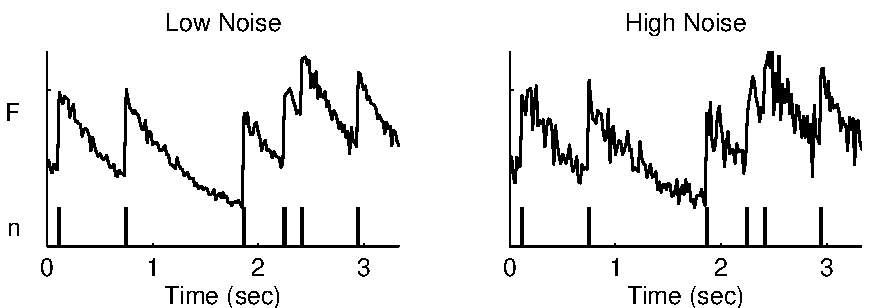
\includegraphics[width=\hsize]{../figs/sim_examples}
\caption{Two example traces of simulated fluorescence data, at
  different SNR levels, demonstrating the relationship between spike
  trains and observed fluorescence in our model.  Note that both
  panels have the same underlying spike train. Simulation parameters:
  $k_i=0.7$, $C_i^b=1$ $\mu$M, $\tau^c_i=500$ msec, $A_i=50$ $\mu$M,
  $\sigma^c_i=0.1$ $\mu$M. $\gamma_i=0.004$ (effective SNR$ \approx
  3$, as defined in Eq.~(\ref{eq:eSNR}); see also Figure
  \ref{fig:recvar-SNR} below) in the left panel and $\gamma_i=0.016$
  (eSNR $\approx 9$) in the right panel, and $\sigma^F_i=0$,
  $\Delta=(60$ Hz$)^{-1}$.}
\label{fig:example_traces}
\end{figure}

To summarize, Eqs.~\eqref{eqn:glm:definition} -- \eqref{eqn:F:definition} define a coupled HMM: the underlying spike trains $\{n_i(t)\}_{i\leq N}$ and spike history terms $\{h_{ij}(t)\}_{i,j\leq N}$ evolve in a Markovian manner given the stimulus $S^{ext}(t)$. These spike trains in turn drive the intracellular calcium concentrations $\{C_i(t)\}_{i\leq N}$, which are themselves Markovian, but evolving at a slower timescale $\tau_i^c$. Finally, we observe only the fluorescence signals $\{F_i(t)\}_{i\leq N}$, which are related in a simple Markovian fashion to the calcium variables $\{C_i(t)\}_{i\leq N}$.


\subsection{Goal and general strategy}  \label{sec:methods:goal}

Our primary goal is to estimate the connectivity matrix, $\bw$, given
the observed set of calcium fluorescence signals $\bF=\{F_i(t)\}_{i
\leq N, t\leq T}$. We must also deal with a number of nuisance
parameters\footnote{The nuisance parameters for neuron $i$ are all its
parameters, minus the cross-coupling terms, i.e.\ $\tbth_i =\bth_i
\backslash \{w_{ij}\}_{i\neq j}$.}, $\tbth_i$: the intrinsic spiking
parameters\footnote{To reduce the notational load, we will ignore the
estimation of the stimulus filter $k_i$ below; this term may be
estimated with $b_i$ and $w_{ii}$ using very similar convex
optimization methods, as discussed in \cite{Vogelstein2009}.}  $\{b_i,
w_{ii}\}_{i\leq N}$, the calcium parameters $\{C^b_i, \tau^c_i, A_i,
\sigma^c_i\}_{i\leq N}$, and the observation parameters $\{\alpha_i,
\beta_i, \gamma_i, \sigma^F_i\}_{i\leq N}$. We addressed the problem
of estimating these nuisance parameters in earlier work
\cite{Vogelstein2009}; thus our focus here will be on the connectivity
matrix $\bw$. A Bayesian approach is natural here, since we have a
good deal of prior information about neural connectivity; see
\cite{Rigat06} for a related discussion. However, a fully-Bayesian
approach, in which we numerically integrate over the very
high-dimensional parameter space $\bth= \{\bth_i\}_{i\leq N}$, where
$\bth_i=\{\bw_i, b_i, C^b_i, \tau^c_i, A_i, \sigma^c_i, \alpha_i,
\beta_i, \gamma_i, \sigma^F_i\}$, is less attractive from a
computational point of view. Thus, our compromise is to compute
\emph{maximum a posteriori} (MAP) estimates for the parameters via an
expectation-maximization (EM) algorithm, in which the sufficient
statistics are computed by a hybrid blockwise Gibbs sampler and
sequential Monte Carlo (SMC) method. More specifically, we iterate the
steps:
\begin{align*}
\textbf{E step} &\text{: Evaluate } Q(\bth,\bth^{(l)}) = E_{P[\bX |
\bF; \bth^{(l)}]} \ln P \left[ \bF, \bX | \bth \right] = \int P[\bX |
\bF; \bth^{(l)}] \ln P[\bF, \bX | \bth] d \bX \\ \textbf{M step}
&\text{: Solve } \bth^{(l+1)} = \argmax_{\bth} \left\{
Q(\bth,\bth^{(l)}) + \ln P(\bth) \right\},
\end{align*}
where $\bX$ denotes the set of all hidden variables $\{ C_i(t), n_i(t), h_{ij}(t) \}_{i,j \leq N, t \leq T}$ and $P(\bth)$ denotes a (possibly improper) prior on the parameter space $\bth$. According to standard EM theory \cite{DLR77,McLachlanKrishnan96}, each iteration of these two steps is guaranteed to increase the log-posterior $\ln P(\bth^{(l)} | \bF)$, and will therefore lead to at least a locally maximum a posteriori estimator.

Now, our major challenge is to evaluate the auxiliary function $Q(\bth,\bth^{(l)})$ in the E-step. Our model is a coupled HMM, as discussed in the previous section; therefore, as usual in the HMM setting \cite{RAB89}, $Q$ may be broken up into a sum of simpler terms:
\begin{eqnarray}
Q(\bth,\bth^{(l)}) &=& \sum_{it} P[C_i(t) | \bF; \bth] \times \ln
P[F_i(t)|C_i(t); \alpha_i, \beta_i, \gamma_i, \sigma^F_i] \nonumber \\
&+& \sum_{it} P[C_i(t), C_i(t-\Delta) | \bF; \bth] \times \ln
P[C_i(t)|C_i(t-\Delta), n_i(t); C^b_i, \tau^c_i, A_i, \sigma^c_i]
\nonumber \\ &+& \sum_{it} P[n_i(t), \bh_i(t) | \bF; \bth] \times \ln
P[n_i(t)| \bh_i(t); b_i, \bw_i]
\label{eqn:loglik:definition-expl}
\end{eqnarray}
\noindent where $\bh_i(t)=\{h_{ij}(t)\}_{j \leq N}$. Note that each of
the three sums here corresponds to a different component of the model
described in Eqs.~\eqref{eqn:glm:definition} --
\eqref{eqn:F:definition}: the first sum involves the fluorescent
observation parameters, the second the calcium dynamics, and the third
the spiking dynamics.

Thus we need only compute low-dimensional marginals of the full
posterior distribution $P[\bX | \bF; \bth]$; specifically, we need
pairwise marginals, of the form $P[C_i(t)| \bF; \bth]$,
$P[n_i(t),\bh_i(t) | \bF; \bth]$, and $P[C_i(t), C_i(t- \Delta) | \bF;
\bth]$.  Details for calculating $P[C_i(t), C_i(t- \Delta) | \bF_i;
\tbth_i]$ and $P[C_i(t)|\bF_i;\tbth_i]$ are found in
\cite{Vogelstein2009}, while calculating the joint marginal for the
high dimensional hidden variable $\bh_i$ necessitates the development
of specialized blockwise Gibbs-SMC sampling methods, as we describe in
the subsequent sections \ref{sec:methods:indep} and
\ref{sec:methods:joint}. Once we have obtained these marginals, the
M-step breaks up into a number of independent optimizations that may
be computed in parallel and which are therefore relatively
straightforward (Section \ref{sec:methods:parameters HMM}); see
section \ref{sec:methods:specific_implementation} for a pseudocode
summary along with some specific implementation details.

\subsection{Initialization of intrinsic parameters via sequential
  Monte Carlo methods} \label{sec:methods:indep}

We begin by constructing relatively cheap, approximate preliminary estimators for the intrinsic parameters, $\tbth_i$.
%= \bth \backslash \{w_{ij}\}_{i\neq j}$, i.e., the observation parameters, $\{\alpha_i,\beta_i,\gamma_i,\sigma^F_i\}$, the calcium dynamics parameters $\{C^b_i,\tau^c_i, A_i, \sigma^c_i\}_i$, and the intrinsic spiking parameters, $\{k_i,b_i,w_{ii}\}$.
The idea is to initialize our estimator by assuming that each neuron
is observed independently. Thus we want to compute $P[C_i(t),
C_i(t-\Delta) | \bF_i; \tbth_i]$ and $P[C_i(t)|\bF_i;\tbth_i]$, and
solve the M-step for each $\tbth_i$, with the connectivity matrix
parameters held fixed. This single-neuron case is much simpler, and
has been discussed at length in \cite{Vogelstein2009}; therefore, we
only provide a brief overview here. The standard forward and backward
recursions provide the necessary posterior distributions, in principle
\cite{ShumwayStoffer06}:
\begin{align}
% \hspace{-25mm}
P[X_i(t) | \bF_i(0:t)] &\propto P[F_i(t)| X_i(t)] \int P[X_i(t) |
    X_i(t-\Delta)] P[X_i(t-\Delta) | \bF_i(0:t-\Delta)] dX_i(t-\Delta),
\label{eqn:forward} \\
% \hspace{-25mm}
P[X_i(t), X_i(t-\Delta) | \bF_i] &= P[X_i(t) | \bF_i]
\frac{P[X_i(t) | X_i(t-\Delta)] P[X_i(t-\Delta) |
\bF_i(0:t-\Delta)]}{\int P[X_i(t) | X_i(t-\Delta)] P[X_i(t-\Delta) |
\bF_i(0:t-\Delta)] dX_i(t-\Delta)},
\label{eqn:backward}
\end{align}
where $\bF_i(s:t)$ denotes the time series $\bF_i$ from time points
$s$ to $t$, and we have dropped the conditioning on the parameters for
brevity's sake. Eq.~\eqref{eqn:forward} describes the forward (filter)
pass of the recursion, and Eq.~\eqref{eqn:backward} describes the
backward (smoother) pass, providing both $P[X_i(t), X_i(t-\Delta) |
\bF_i]$ and $P[X_i(t) | \bF_i]$ (obtained by marginalizing over
$X_i(t-\Delta)$).

Because these integrals cannot be analytically evaluated for our
model, we approximate them using a SMC (``marginal particle
filtering'') method \cite{DGA00,DFG01,GDW04}; see
\cite{Vogelstein2009} for details on the proposal density and
resampling methods used here. The output of this SMC method comprises
an array of particle positions $\{X_i^{(m)}(t)\}_{m=1}^{M}$, where $m$
indexes the particle number and $M$ the total number of particles ($M$
was typically set to about $50$ in our experiments), and a discrete
approximation to the marginals $P[X_i(t), X_i(t-\Delta) | F_i]$,
\begin{multline}
% \begin{array}{rl}
P[X_i(t), X_i(t-\Delta) | F_i] \\ \approx \sum_{m,m'}
r_i^{(m,m')}(t,t-\Delta) \delta \left[ X_i(t) - X_i^{(m)}(t) \right]
\delta \left[ X_i(t-\Delta) - X_i^{(m')}(t-\Delta) \right],
% \end{array}
\label{eqn:particle-fb}
\end{multline}
where $r_i^{(m,m')}(t,t-\Delta)$ denotes the weight attached to the
pair of particles with positions $\left( X_i^{(m)}(t),
X_i^{(m')}(t-\Delta) \right)$, and $\delta(.)$ denotes a Dirac mass.
Thus equations (\ref{eqn:forward}-\ref{eqn:particle-fb}) may be used
to compute the the sufficient statistics for estimating the
intrinsic parameters $\tbth_i$ for each neuron. 

As discussed following Eq.~\eqref{eqn:loglik:definition-expl}, the
M-step decouples into three independent subproblems. The first term
depends on only $\{\alpha_i, \beta_i, \gamma_i, \sigma_i\}$; since
$P[F_i(t)|S(C_i(t)); \tbth_i]$ is Gaussian, we can estimate these
parameters by solving a weighted regression problem (specifically, we
use a coordinate-optimization approach: we solve a quadratic problem
for $\{\alpha_i, \beta_i\}$ while holding $\{\gamma_i, \sigma_i\}$
fixed, then estimate $\{\gamma_i,\sigma_i\}$ by the usual residual
error formulas while holding $\{\alpha_i, \beta_i\}$
fixed). Similarly, the second term requires us to optimize over
$\{\tau_i^c, A_i, C_i^b\}$, and then we use the residuals to estimate
$\sigma_i^c$. Note that all the parameters mentioned so far are
constrained to be non-negative, but may be solved efficiently using
standard quadratic program solvers if we use the simple
reparameterization $\tau_i^c \to 1- \Delta / \tau_i^c$. Finally, the
last term may be expanded:
\begin{multline}
E [\ln P[n_i(t), \bh_i(t) | \bF; \bth_i]] \\ = P[n_i(t), \bh_i(t) |
\bF] \ln f [J_i(t)] + (1-P[n_i(t), \bh_i(t) | \bF]) \ln [1-
f(J_i(t))];
\label{eqn:bw}
\end{multline}
since $J_i(t)$ is a linear function of $\{b_i,\bw_i\}$, and the
right-hand side of Eq.~\eqref{eqn:bw} is concave in $J_i(t)$, we see
that the third term in Eq.~\eqref{eqn:loglik:definition-expl} is a sum
of terms which are concave in $\{b_i,\bw_i\}$ --- and therefore also
concave in the linear subspace $\{b_i,w_{ii}\}$ with $\{w_{ij}\}_{i
\neq j}$ held fixed --- and may thus be maximized efficiently using
any convex optimization method, e.g.\ Newton-Raphson or conjugate
gradient ascent.

Our procedure therefore is to initialize the parameters for each
neuron using some default values that we have found to be effective in
practice in analyzing real data, and then iteratively (i) estimate the
marginal posteriors via the SMC recursions
(Eqs.~\ref{eqn:forward}-\ref{eqn:particle-fb}) (E step), and (ii)
maximize over the intrinsic parameters $\tbth_i$ (M step), using the
separable convex optimization approach described above. We iterate
these two steps until the change in $\tbth_i$ does not exceed some
minimum threshold. We then use the marginal posteriors from the last
iteration to seed the blockwise Gibbs sampling procedure described
below for approximating $P[n_i,\bh_i | \bF;\bth_i]$.

\subsection{Estimating joint posteriors over weakly coupled neurons}
\label{sec:methods:joint}

Now we turn to the key problem: constructing an estimate of the joint
marginals $\{P[n_i(t), \bh_i(t) | \bF;\bth]\}_{i\leq N}$, which are
the sufficient statistics for estimating the connectivity matrix $\bw$
(recall Eq.~\eqref{eqn:loglik:definition-expl}). The SMC method
described in the preceding section only provides the marginal
distribution over a single neuron's hidden variables; this method may
in principle be extended to obtain the desired full posterior
$P[\bX(t), \bX(t-\Delta) | \bF; \bth]$, but SMC is fundamentally a
sequential importance sampling method, and therefore scales poorly as
the dimensionality of the hidden state $\bX(t)$ increases
\cite{BickelBengtsson08}. Thus we need a different approach.

One very simple idea is to use a Gibbs sampler: sample sequentially
from
\begin{align}
X_i(t) \sim P[X_i(t) | \bX_{\i}, X_i(0), \ldots, X_i(t-\Delta),
 X_i(t+\Delta), \ldots, X_i(T), \bF; \bth],
\end{align}
looping over all cells $i$ and all time bins $t$. Unfortunately, this approach is likely to mix poorly, due to the strong temporal dependence between $X_i(t)$ and $X_i(t+\Delta)$. Instead, we propose a blockwise Gibbs strategy, sampling one spike train as a block:
\begin{align}
	\bX_i \sim P[\bX_i | \bX_{\i}, \bF; \bth].
\end{align}
If we can draw these blockwise samples $\bX_i = \bX_i(s:t)$
efficiently for a large subset of $t-s$ adjacent time-bins
simultaneously, then we would expect the resulting Markov chain to mix
much more quickly than the single-element Gibbs chain.  This follows
due to the weak dependence between $\bX_i$ and $\bX_j$ when $i\neq j$,
and the fact that Gibbs is most efficient for weakly-dependent
variables \cite{RC05}.

So, how can we efficiently sample from $P[\bX_i | \bX_{\i}, \bF;
\bth]$? One attractive approach is to try to re-purpose the SMC method
described above, which is quite effective for drawing approximate
samples from $P[\bX_i | \bX_{\i}, \bF_i; \bth]$ for one neuron $i$ at
a time. Recall that sampling from an HMM is in principle easy by the
``propagate forward, sample backward'' method: we first compute the
forward probabilities $P[X_i(t) | \bX_{\i}(0:t), \bF_i(0:t); \bth]$
recursively for timesteps $t=0$ up to $T$, then sample backwards from
$P[X_i(t) | \bX_{\i}(0:T), \bF_i(0:T), X_i(t-\Delta); \bth]$. This
approach is powerful because each sample requires just linear time to
compute (i.e., $O(T/\Delta)$ time, where $T/\Delta$ is the number of
desired time steps). Unfortunately, in this case we can only compute
the forward probabilities approximately (with the SMC forward
recursion approximation to Eq.~\eqref{eqn:forward}), and so therefore
this attractive forward-backward approach only provides approximate
samples from $P[\bX_i | \bX_{\i}, \bF; \bth]$, not the exact samples
required for the validity of the Gibbs method.

Of course, in principle we should be able to use the
Metropolis-Hastings (M-H) algorithm to correct these approximate
samples. The problem is that the M-H acceptance ratio in this setting
involves a high-dimensional integral over the set of paths that the
particle filter might possibly trace out, and is therefore difficult
to compute directly. \cite{Andrieu2007} discuss this problem at more
length, along with some proposed solutions. A slightly simpler
approach was introduced by \cite{NBR03}. Their idea is to exploit the
$O(T/\Delta)$ forward-backward sampling method by embedding a discrete
Markov chain within the continuous state space $\mathcal{X}_t$ on
which $X_i(t)$ is defined; the state space of this discrete embedded
chain is sampled randomly according to some distribution $\rho_t$ with
support on $\mathcal{X}_t$. It turns out that an appropriate
acceptance probability (defined in terms of the original state space
model transition and observation probabilities, along with the
auxiliary sampling distributions $\rho_t$) may be computed quite
tractably, guaranteeing that the samples produced by this algorithm
form a Markov chain with the desired equilibrium density. See
\cite{NBR03} for details.

We can apply this embedded-chain method quite directly here to sample
from $P[\bX_i | \bX_{\i}, \bF; \bth]$. The one remaining question is
how to choose the auxiliary densities $\rho_t$. We would like to
choose these densities to be close to the desired marginal densities
$P[X_i(t) | \bX_{\i}, \bF; \bth]$, and conveniently, we have already
computed a good (discrete) approximation to these densities, using the
SMC methods described in the last section. The algorithm described in
\cite{NBR03} requires the densities $\rho_t$ to be continuous, so we
simply convolve our discrete SMC-based approximation (specifically,
the $X_i(t)$-marginal of Eq.~\eqref{eqn:particle-fb}) with an
appropriate normal density to arrive at a very tractable
mixture-of-Gaussians representation for $\rho_t$.

Thus, to summarize, our procedure for approximating the desired joint
state distributions $P[n_i(t), \bh_i(t) | \bF;\bth_i]$ has a
Metropolis-within-blockwise-Gibbs flavor, where the internal
Metropolis step is replaced by the $O(T/\Delta)$ embedded-chain method
introduced by \cite{NBR03}, and the auxiliary densities $\rho_t$
necessary for implementing the embedded-chain sampler are obtained
using the SMC methods from \cite{Vogelstein2009}.

\subsubsection{A factorized approximation of the joint posteriors}
\label{sec:cheaper-high-snr}

If the SNR in the calcium imaging is sufficiently high, then by
definition the observed fluorescence data $\bF_i$ will provide enough
information to determine the underlying hidden variables
$\bX_i$. Thus, in this case the joint posterior approximately
factorizes into a product of marginals for each neuron $i$:
\begin{equation} \label{eqn:indep_approx}
  P[\bX|\bF;\bth] \approx \prod_{i\leq N} P[\bX_i | \bF; \tbth_i].
\end{equation}
We can take advantage of this because we have already estimated all
the marginals on the right hand side using the approximate SMC methods
in Section \ref{sec:methods:indep}.  This factorized approximation
entails a very significant gain in efficiency for two reasons: first,
it obviates the need to generate joint samples via the expensive
blockwise-Gibbs approach described above; and second, because we can
very easily parallelize the SMC step, inferring the marginals
$P[X_i(t) | F_i; \tbth_i]$ and estimating the parameters $\bth_i$ for
each neuron on a separate processor. We will discuss the empirical
accuracy of this approximation in the Results section.

\subsection{Estimating the functional connectivity matrix} \label{sec:methods:parameters HMM}

Computing the M-step for the connectivity matrix, $\bw$, is an optimization problem with on the order of $N^2$ variables. The auxiliary function Eq.~\eqref{eqn:loglik:definition-expl} is concave in $\bw$, and decomposes into $N$ separable terms that may be optimized independently using standard ascent methods. To improve our estimates, we will incorporate two sources of strong \emph{a priori} information via our prior $P(\bw)$: first, previous anatomical studies have established that connectivity in many neuroanatomical substrates is ``sparse,'' i.e., most neurons form synapses with only a fraction of their neighbors \cite{Buhl94,Thompson88,Reyes98,Feldmeyer99,Gupta00,FeldmeyerSakmann00,PetersenSakmann00,Binzegger04,Song2005,Mishchenko2009b}, implying that many elements of the connectivity matrix $\bw$ are zero; see also \cite{PAN04c,Rigat06,PILL07,Stevenson08} for further discussion. Second, ``Dale's law'' states that each of a neuron's postsynaptic connections in adult cortex (and many other brain areas) must all be of the same sign (either excitatory or inhibitory). Both of these priors are easy to incorporate in the M-step optimization, as we discuss below.


\subsubsection{Imposing a sparse prior on the functional connectivity}

It is well-known that imposing sparseness via an $L1$-regularizer can
dramatically reduce the amount of data necessary to accurately
reconstruct sparse high-dimensional parameters
\cite{Tibs96,TIP01,DE03,NG04,Candes2005,Mishchenko2009}. We
incorporate a prior of the form $\ln p(\bw) = const. - \lambda
\sum_{i,j} |\w_{ij}|$, and additionally enforce the constraints
$|\w_{ij}|<L$, for a suitable constant $L$ (since both excitatory and
inhibitory cortical connections are known to be bounded in
size). Since the penalty $\ln p(\bw)$ is concave, and the constraints
$|\w_{ij}|<L$ are convex, we may solve the resulting optimization
problem in the M-step using standard convex optimization methods
\cite{CONV04}. In addition, the problem retains its separable
structure: the full optimization may be broken up into $N$ smaller
problems that may be solved independently.

\subsubsection{Imposing Dale's law on the functional connectivity}

Enforcing Dale's law requires us to solve a non-convex, non-separable
problem: we need to optimize the concave function $Q(\bth,\bth^{(l)})
+ \ln P(\bth)$ under the non-convex, non-separable constraint that all
of the elements in any column of the matrix $\bw$ are of a definite
sign (either nonpositive or nonnegative). It is difficult to solve
this nonconvex problem exactly, but we have found that simple greedy
methods are quite efficient in finding good approximate solutions.

We begin with our original sparse solution, obtained as discussed in
the previous subsection without enforcing Dale's law. Then we assign
each neuron as either excitatory or inhibitory, based on the weights
we have inferred in the previous step: i.e., neurons $i$ whose
inferred postsynaptic connections $w_{ij}$ are largely positive are
tentatively labeled excitatory, and neurons with largely inhibitory
inferred postsynapic connections are labeled inhibitory. Neurons which
are highly ambiguous may be unassigned in the early iterations, to
avoid making mistakes from which it might be difficult to
recover. Given the assignments $a_i$ ($a_i =1$ for putative excitatory
cells, $-1$ for inhibitory, and $0$ for neurons which have not yet
been assigned) we solve the convex, separable problem \begin{equation}
\argmax_{\substack{a_i \w_{ij} \geq 0, |w_{ij}|<L ~ \forall i,j}}
Q(\bth,\bth^{(l)}) - \lambda \sum_{ij} |w_{ij}| \end{equation} which
may be handled using the standard convex methods discussed
above. Given the new estimated connectivities $\bw$, we can re-assign
the labels $a_i$, or flip some randomly to check for local optima. We
have found this simple approach to be effective in practice.


\subsection{Specific implementation notes} \label{sec:methods:specific_implementation}

Pseudocode summarizing our approach is given in Algorithm \ref{eqn:pseudocode}. As discussed in Section \ref{sec:methods:indep}, the intrinsic parameters $\tbth_i$ may be initialized effectively using the methods described in \cite{Vogelstein2009}; then the full parameter $\bth$ is estimated via EM, where we use the embedded-chain-within-blockwise-Gibbs approach discussed in Section \ref{sec:methods:joint} (or the cheaper factorized approximation described in Section \ref{sec:cheaper-high-snr}) to obtain the sufficient statistics in the E step and the separable convex optimization methods discussed in Section \ref{sec:methods:parameters HMM} for the M step.

\begin{algorithm}[t!]
\caption{Pseudocode for estimating functional connectivity from
calcium imaging data using EM; $\eta_1$ and $\eta_2$ are
user-defined convergence tolerance parameters.}
\label{eqn:pseudocode}
\begin{algorithmic}
\While{$|{\bw}^{(l)}-{\bw}^{(l-1)}|>\eta_1$}
  \ForAll{$i=1\ldots N$}
    \While{$|{\tbth_i}^{(l)}-{\tbth_i}^{(l-1)}|> \eta_2$}
      \State Approximate $P[X_i(t)|F_i; \tbth_i]$ using SMC (Section \ref{sec:methods:indep})
      \State Perform the M-step for the intrinsic parameters $\tbth_i$ (Section \ref{sec:methods:indep})
    \EndWhile
  \EndFor
      \ForAll{$i=1\ldots N$}
      \State Approximate $P[n_i(t), \bh_i(t) |\bF; \bth_i]$ using either the blockwise Gibbs
      \State method or the factorized approximation (Section \ref{sec:methods:joint})
    \EndFor
  \ForAll{$i=1\ldots N$}
  	\State Perform the M-step using separable convex optimization methods (Section \ref{sec:methods:parameters HMM})
  \EndFor
\EndWhile
\end{algorithmic}
\end{algorithm}

As emphasized above, the parallel nature of these EM steps is
essential for making these computations tractable. We performed the
bulk of our analysis on a 256-processor cluster of Intel Xeon L5430
based computers (2.66 GHz). For 10 minutes of simulated fluorescence
data, imaged at $30$ Hz, calculations using the factorized
approximation typically took 10-20 minutes per neuron (divided by the
number of available processing nodes on the cluster), with time split
approximately equally between (i) estimating the intrinsic parameters
$\tbth_i $, (ii) approximating the posteriors using the independent
SMC method, and (iii) estimating the functional connectivity matrix,
$\bw$. The hybrid embedded-chain-within-blockwise-Gibbs sampler was
substantially slower, up to an hour per neuron, with the Gibbs sampler
dominating the computation time, because we thinned the chain by a
factor of five, following preliminary quantification of the
autocorrelation timescale of the Gibbs chain (data not shown).


\subsection{Simulating a neural population} \label{sec:results:simulations}

To test the described method for inferring functional connectivity
from calcium imaging data, we simulated networks (according to our
model, Eqs.~\eqref{eqn:glm:definition} -- \eqref{eqn:F:definition}) of
spontaneously firing randomly connected neurons. Although simulations
ran at $1$ msec time discretization, the imaging rate was assumed to
be much slower: $5$--$200$ Hz (c.f.~Fig.~\ref{fig:recvar} below).

Model parameters were chosen based on experimental data available in
the literature for cortical neural networks
\cite{Braitenberg1998,Urquijo2000,Lefort2009,Sayer1990}. More
specifically, the network consisted of 80\% excitatory and 20\%
inhibitory neurons \cite{Braitenberg1998,Urquijo2000}, each respecting
Dale's law (as discussed in section \ref{sec:methods:parameters HMM}
above). Neurons were randomly connected to each other in a spatially
homogeneous manner with probability $0.1$
\cite{Braitenberg1998,Lefort2009}. Synaptic weights for excitatory
connections, as defined by excitatory postsynaptic potential (PSP)
peak amplitude, were randomly drawn from an exponential distribution
with the mean of $0.5$ mV \cite{Lefort2009,Sayer1990}. Inhibitory
connections were also drawn from an exponential distribution; their
strengths chosen so as to balance excitatory and inhibitory currents
in the network, and achieve an average firing rate of $\approx 5 $ Hz
\cite{Abeles91}. Practically, this meant that the mean strength of
inhibitory connections was about 10 times larger than that of the
excitatory connections. PSP shapes were modeled as an alpha function
\cite{Koch99}: roughly, the difference of two exponentials,
corresponding to a sharp rise and relatively slow decay
\cite{Sayer1990}. We neglected conduction delays, given that the time
delays below $\sim 1$ msec expected in the local cortical circuit were
far below the time resolution of our simulated imaging data.

Note that PSP peak amplitudes measured \emph{in vitro} (as in, e.g.,
\cite{Song2005}) cannot be incorporated directly in
Eq.~\eqref{eqn:glm:definition}, since the synaptic weights in our
model --- $w_{ij}$ in Eq.~\eqref{eqn:glm:definition} --- are
dimensionless quantities representing the change in the spiking
probability of neuron $i$ given a spike in neuron $j$, whereas PSP
peak amplitude describes the physiologically measured change in the
membrane voltage of a neuron due to synaptic currents triggered by a
spike in neuron $j$.  To relate the two, note that in order to trigger
an immediate spike in a neuron that typically has its membrane voltage
$V_b$ mV below the spiking threshold, roughly $n_E = V_b / V_E$
simultaneous excitatory PSPs with the peak amplitude $V_E$ would be
necessary.  Therefore, the change in the spiking probability of a
neuron due to excitatory synaptic current $V_E$ can be approximately
defined as (so that $\delta P_E n_E \approx 1$)
\begin{equation}\label{eqn:convert:leadin-1}
\delta P_E = V_E/V_b.
\end{equation}
$V_b \approx 15$ mV here, while values for the PSP amplitude $V_E$
were chosen as described above.  Similarly, according to
Eq.~\ref{eqn:glm:definition}, the same change in the spiking
probability of a neuron $i$ following the spike of a neuron $j$ in the
GLM is roughly
\begin{equation}\label{eqn:convert:leadin-2}
\delta P_E = \left[ f(b_i + w_{ij}) - f(b_i) \right] \tau_h,
\end{equation}
where recall $\tau_h$ is the typical PSP time-scale, i.e. the time
over which a spike in neuron $j$ significantly affects the firing
probability of the neuron $i$.  Equating these two expressions gives
us a simple method for converting the physiological parameters $V_E$
and $V_b$ into suitable GLM parameters $w_{ij}$.

Finally, parameters for the internal calcium dynamics and fluorescence
observations were chosen according to our experience with several
cells analyzed using algorithm of \cite{Vogelstein2009}, and conformed
to previously published results
\cite{ImagingManual,HelmchenSakmann96,BrenowitzRegehr07}. Table
\ref{table:caparm} summarizes the details for each of the parameters
in our model.

\begin{table}[h!b!p!]
\caption{Table of simulation parameters. $\mathcal{E}(\lambda)$
indicates an exponential distribution with mean $\lambda$, and
$\mathcal{N}_p(\mu,\sigma^2)$ indicates a normal distribution with
mean $\mu$ and variance $\sigma^2$, truncated at lower bound $p\mu$.
Units (when applicable) are given with respect to mean values (i.e.,
units are squared for variance).}\label{table:caparm}

\begin{tabular}{lll}
\hline
Total neurons & 10-500 & \# \\
Excitatory neurons & $80$ & $\%$ \\
Connections sparseness & $10$   & $\%$ \\
Baseline firing rate & $5$ & Hz\\
\hline
Excitatory PSP peak height 	& $\sim \mathcal{E}(0.5)$ & mV \\
Inhibitory PSP peak height 	& $\sim -\mathcal{E}(2.3)$ & mV \\
Excitatory PSP rise time 		& 1 & msec \\
Inhibitory PSP rise time 		& 1 & msec \\
Excitatory PSP decay time 	& $\sim \mathcal{N}_{0.5}(10,2.5)$ & msec \\
Inhibitory PSP decay time 	& $\sim \mathcal{N}_{0.5}(20,5)$ & msec\\
Refractory time, $w_{ii}$ 	& $\sim \mathcal{N}_{0.5}(10,2.5)$ & msec \\
\hline
Calcium std. $\sigma_c$ & $\sim \mathcal{N}_{0.4}(28,10)$ & $\mu$M\\
Calcium jump after spike, $A_c$ &  $\sim \mathcal{N}_{0.4}(80,20)$ & $\mu$M\\
Calcium baseline, $C_b$ & $\sim \mathcal{N}_{0.4}(24,8)$ & $\mu$M\\
Calcium decay time, $\tau_c$ & $\sim \mathcal{N}_{0.4}(200,60)$ & msec\\
Dissociation constant, $K_d$ & $200$ & $\mu$M \\
\hline
Fluorescence scale, $\alpha$ & $1$ & n/a\\
Fluorescence baseline, $\beta$ & $0$ &  n/a\\
Signal-dependent noise, $\gamma$ & $10^{-3}$-$10^{-5}$ & n/a\\
Signal-independent noise, $\sigma^F$ & $4\cdot 10^{-3}$-$4\cdot 10^{-5}$ & n/a\\
\end{tabular}
\end{table}

\section{Results}
\label{sec:results}

In this section we study the performance of our proposed network
estimation methods, using the simulated data described in section
\ref{sec:results:simulations} above.  Specifically, we estimated the
connectivity matrix using both the
embedded-chain-within-blockwise-Gibbs approach and the simpler
factorized approximation.  Figure \ref{fig:scatters} summarizes one
typical experiment: the EM algorithm using the factorized
approximation estimated the connectivity matrix about as accurately as
the full embedded-chain-within-blockwise-Gibbs approach ($r^2=0.47$
versus $r^2=0.48$).  Thus in the following we will focus primiarily on
the factorized approximation, since this is much faster than the full
blockwise-Gibbs approach (recall section
\ref{sec:methods:specific_implementation}).

\begin{figure}[t!]
\centering
\begin{minipage}[c]{0.45\hsize}
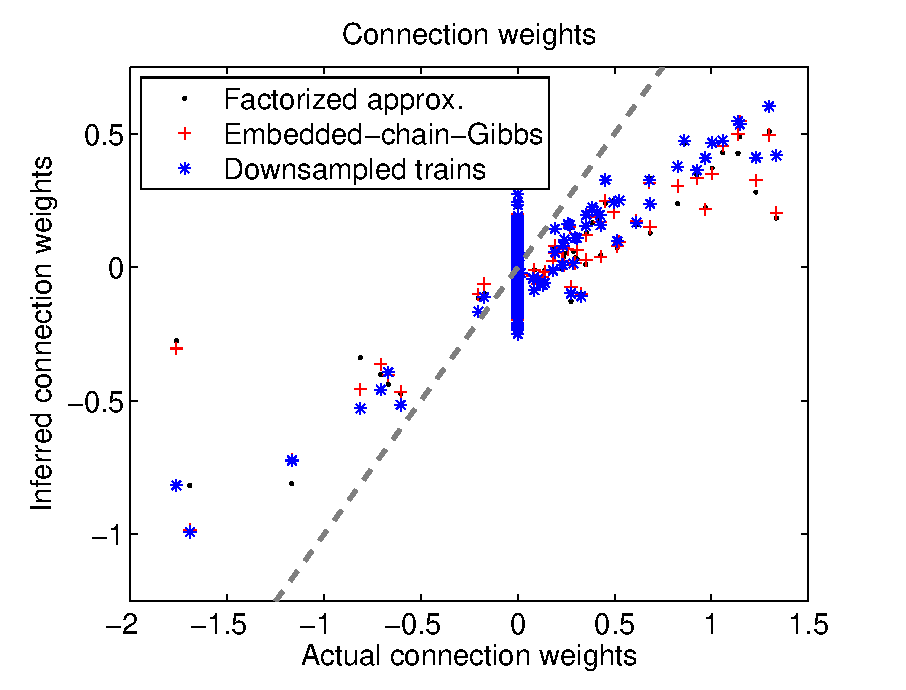
\includegraphics[width=\hsize]{../figs/FigureA3_scatter_three}
\end{minipage}
\begin{minipage}[c]{0.45\hsize}
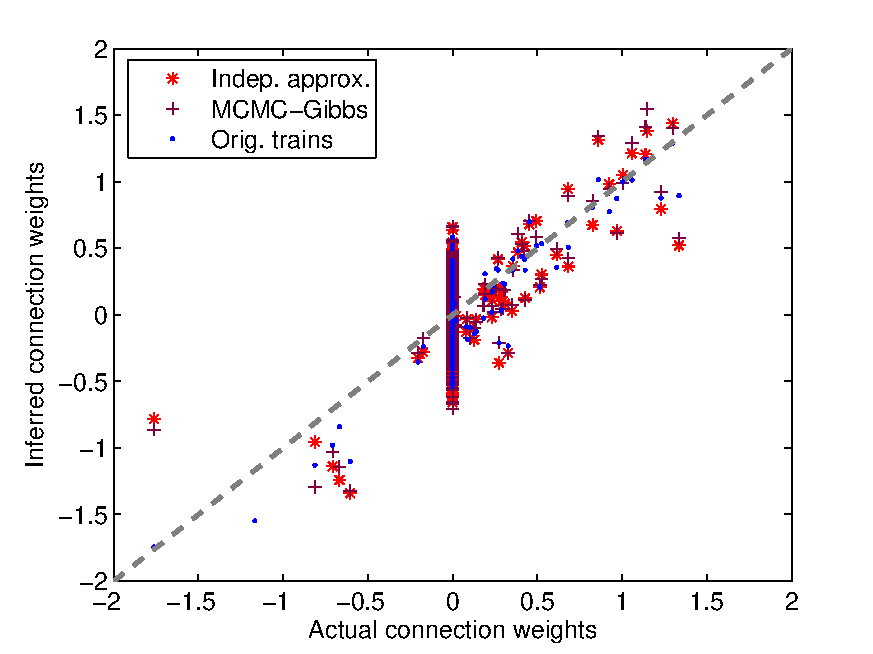
\includegraphics[width=\hsize]{../figs/FigureA3_scatter_three_corrected}
\end{minipage}
\caption{Quality of the connectivity matrix estimated from simulated
calcium imaging data. Inferred connection weights $\hat w_{ij}$ are
shown in a scatter plot versus real connection weights $w_{ij}$, with
inference performed using the factorized approximation, exact
embedded-chain-within-blockwise-Gibbs approach, and true spike trains
down-sampled to the frame rate of the calcium imaging. A network of
$N=25$ neurons was used, firing at $\approx 5$ Hz, and imaged for
$T=10$ min at intermediate eSNR $\approx 6$ (see eq.~(\ref{eq:eSNR})
and Figure \ref{fig:recvar-SNR} below).  The squared correlation
coefficient between the connection weights calculated using factorized
approximation and true connection weights was $r^2=0.47$, compared
with the embedded-chain-within-blockwise-Gibbs method's
$r^2=0.48$. For connection weights calculated directly from the true
spike train down-sampled to the calcium imaging frame rate we obtained
$r^2=0.57$.  Here and in the following figures the gray dashed line
indicates unity, $y=x$.  The inferred connectivity in the left panel
shows a clear scale bias, which can be corrected by dividing by the
scale correction factor calculated in section \ref{sec:scale} below
(right panel).  The vertical lines apparent at zero in both subplots
are due to the fact that the connection probability in the true
network was significantly less than one: i.e., many of the true
weights $w_{ij}$ are exactly zero.}
\label{fig:scatters} \end{figure}


\subsection{Impact of coarse time discretization of calcium imaging
  data and scale factor of inferred connection weights}
\label{sec:scale}

A notable feature of the results illustrated in the left panel of
Fig.~\ref{fig:scatters} is that our estimator is biased downwards by a
roughly constant scale factor: our estimates $\hat w_{ij}$ are
approximately linearly related to the true values of $w_{ij}$ in the
simulated network, but the slope of this linear relationship is less
than one.  At first blush, this bias does not seem like a major
problem: as we discussed in section \ref{sec:results:simulations},
even in the noiseless case we should at best expect our estimated
coupling weights $\hat w_{ij}$ to correspond to some monotonically
increasing function of the true neural connectivities, as measured by
biophysical quantities such as the peak PSP amplitude.  Nonetheless,
we would like to understand the source of this bias more
quantitatively; in this section, we discuss this issue in more depth
and derive a simple method for correcting the bias.

The bias is largely due to the fact that we suffer a loss of temporal
resolution when we attempt to infer spike times from slowly-sampled
fluorescence data.  As discussed in \cite{Vogelstein2009}, we can
recover some of this temporal information by using a finer time
resolution for our recovered spike trains than $\Delta$, the time
resolution of the observed fluorescence signal.  However, when we
attempted to infer $\bw$ directly spike trains sampled from the
posterior $P[\bX|\bF]$ at higher-than-$\Delta$ resolution, we found
that the inferred connectivity matrix was strongly biased towards the
symmetrized matrix $(\bw+\bw^T)/2$ (data not shown).  In other words,
whenever a nearly synchronous jump was consistently observed in two
fluorescent traces $F_i(t)$ and $F_j(t)$ (at the reduced time
resolution $\Delta$), the EM algorithm would typically infer an
excitatory \emph{bidirectional} connection: i.e., both $\hat w_{ij}$
and $\hat w_{ji}$ would be large, even if only a unidirectional
connection existed between neurons $i$ and $j$ in the true network.
While we expect, by standard arguments, that the Monte Carlo EM
estimator constructed here should be consistent (i.e., we should
recover the correct $\bw$ in the limit of large data length $T$ and
many Monte Carlo samples), we found that this bias persisted given
experimentally-reasonable lengths of data and computation time.

Therefore, to circumvent this problem, we simply used the original
imaging time resolution $\Delta$ for the inferred spike trains: note
that, due to the definition of the spike history terms $h_{ij}$ in
equation (\ref{eqn:h:definition}), a spike in neuron $j$ at time $t$
will only affect neuron $i$'s firing rate at time $t+\Delta$ and
greater.  This successfully counteracted the symmetrization problem
(and also sped the calculations substantially), but resulted in the
scale bias exhibited in Figure \ref{fig:scatters}, since any spikes
that fall into the same time bin are treated as coincidental: only
spikes that precede spikes in a neighboring neuron by at least one
time step will directly affect the estimates of $w_{ij}$, and
therefore grouping asynchronous spikes within a single time bin
$\Delta$ results in a loss of information.

To estimate the magnitude of this time-discretization bias more
quantitatively, we consider a significantly simplified case of two
neurons coupled with a small weight $w_{12}$, and firing with baseline
firing rate of $r=f(b)$.  In this case an approximate sufficient
statistic for estimating $w_{12}$ may be defined as:
\begin{equation}\label{eqn:scale:leadin-1}
\begin{array}{rl}
SS ~ =& E\left[\int\limits_{t'}^{t'+\mathcal{T}} n_1(t) dt ~ \bigg| ~
n_2(t')=1, n_2(t)=0 ~ \forall
t \in (t',t'+\mathcal{T}] \right] \\ \approx & r
\mathcal{T} + f'(b) w_{12}\tau_h.
\end{array}
\end{equation}
This leads to a conceptually simple method-of-moments estimator,
\begin{equation}\label{eqn:scale:leadin-2}
\hat w_{12}=(SS-r\mathcal{T})/f'(b)\tau_h.
\end{equation}
Now, if the spike trains are down-sampled into time-bins of size $\Delta$,
we must estimate the statistic $SS$ with a discrete sum instead:
\begin{equation}\label{eqn:scale:leadin-3}
\begin{array}{rl}
SS^{ds} ~ = &E\left[\sum\limits_{t=t'+\Delta}^{t'+\Delta +
  \mathcal{T}} n^{ds}_1(t) ~ \bigg| ~ n^{ds}_2(t')=1, n^{ds}_2(t)=0\
  \forall t \in (t',t'+\mathcal{T}] \right] \\ \approx& r \mathcal{T}
  + f'(b) \int\limits_0^\Delta \frac{dt'}{\Delta}
  \int\limits_{\Delta}^{\Delta + \mathcal{T}}
  w_{12}\exp(-(t-t')/\tau_h) dt \\ \approx & r \mathcal{T} +
  f'(b)w_{12}\frac{1-\exp(-\Delta/\tau_h)}{\Delta/\tau_h^2}.
\end{array}
\end{equation}
$n^{ds}(t)$ here are down-sampled spikes, i.e. the spikes defined on a
grid $t=0,\Delta,2\Delta,\ldots$.  In the second equality we made the
approximation that the true position of the spike of the second
neuron, $n^{ds}_2(t')$, may be uniformly distributed in the first
time-bin $[0,\Delta]$, and the discrete sum over $t$ is from the
second time-bin $[\Delta,2\Delta]$ to
$[\mathcal{T},\mathcal{T}+\Delta]$, i.e. over all spikes of the first
neuron that occurred in any of the strictly subsequent time-bins up to
$\mathcal{T} + \Delta$.  Forming a method-of-moments estimator as in
Eq.~\ref{eqn:scale:leadin-2} leads to a biased estimate:
\begin{equation}\label{eqn:bias}
\hat w_{12}^{ds}\approx \frac{1-\exp(-\Delta/\tau_h)}{\Delta/\tau_h}
\hat w_{12},
\end{equation}
and somewhat surprisingly (given the crude nature of this argument),
this corresponds quite well with the scale bias we observe in
practice.  In Figure \ref{fig:bias} we plot the scale bias from
Eq.~\ref{eqn:bias} versus that empirically deduced from our
simulations for different values of $\Delta$.  As can be seen in
Figure \ref{fig:bias}, Eq. \ref{eqn:bias} describes the observed scale
bias fairly well.  Thus we can divide by this analytically-derived
factor to effectively correct the bias of our estimates, as shown in
the right panel of Fig.~\ref{fig:scatters}.


\begin{figure}[t!]
\centering
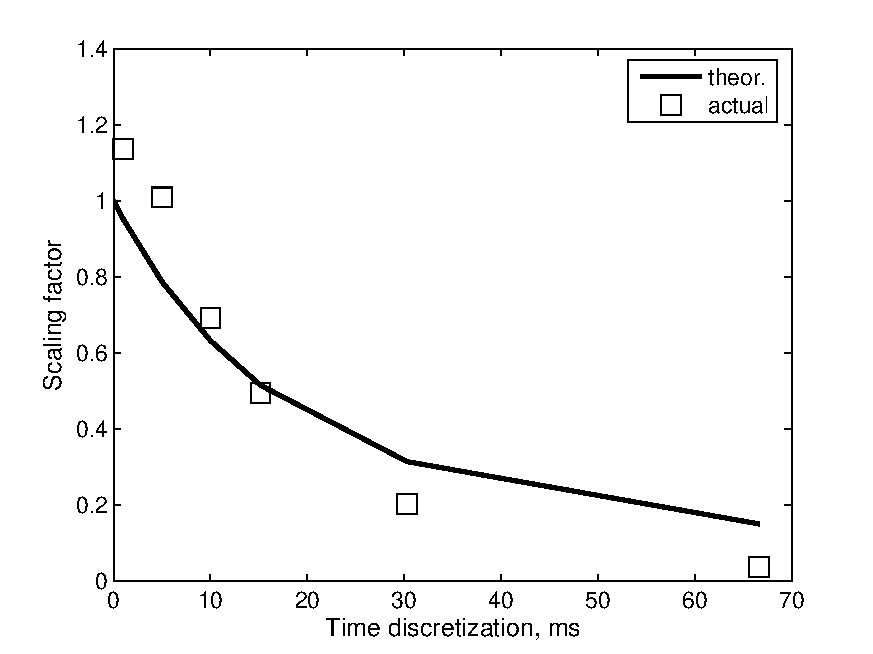
\includegraphics[width=3in]{../figs/FigureA4_scale_bias}
\caption{The low frame rate of calcium imaging explains the scale
error observed in the inferred connectivity weights shown in Figure
\ref{fig:scatters}.  A correction scale factor may be calculated
analytically (thick line) as discussed in the main text
(eq.~\ref{eqn:bias}).  The scale error observed empirically (thin
line) matches well with such theoretical estimate. In the latter case,
the scale error was calculated from the fits obtained directly from
the true spike trains, down sampled to different $\Delta$, for a
network of $N=25$ neurons firing at $\approx 5$ Hz and observed for
$T=10$ min. The error-bars indicate 95\% confidence intervals for
scale error at each $\Delta$.}
\label{fig:bias}
\end{figure}

\subsection{Impact of prior information on the inference}

Next we investigated the importance of incorporating prior information
in our estimates.  We found that imposing a sparse prior (as described
in section \ref{sec:methods:parameters HMM}) significantly improved
our results.  For example, Fig.~\ref{fig:sparse} illustrates a case in
which our obtained $r^2$ increased from $0.64$ (with no L$_1$
penalization in the M-step) to $0.85$ (with penalization; the penalty
$\lambda$ was chosen approximately as the inverse mean absolute value
of $w_{ij}$, which is known here because we prepared the network
simulations but is available in practice given the previous
physiological measurements discussed in section
\ref{sec:results:simulations}).  See also Fig.~\ref{fig:recvar-NT}
below.  Furthermore, the weights estimated using the sparse prior more
reliably provide the sign (i.e., exicitatory or inhibitory) of each
presynaptic neuron in the network (Figure \ref{fig:distros}); the
right panel of Figure \ref{fig:distros} illustrates that our method
infers the sign of presynaptic neurons with high accuracy.

Incorporation of Dale's law, on the other hand, only leads to an
$\approx 10\%$ change in the estimation $r^2$ in the absence of an
L$_1$ penalty, and no significant improvement at all in the presence
of an L$_1$ penalty (data not shown).  Thus Dale's prior was not
pursued further here.

\begin{figure}[t!]
\centering
\begin{minipage}[c]{0.45\hsize}
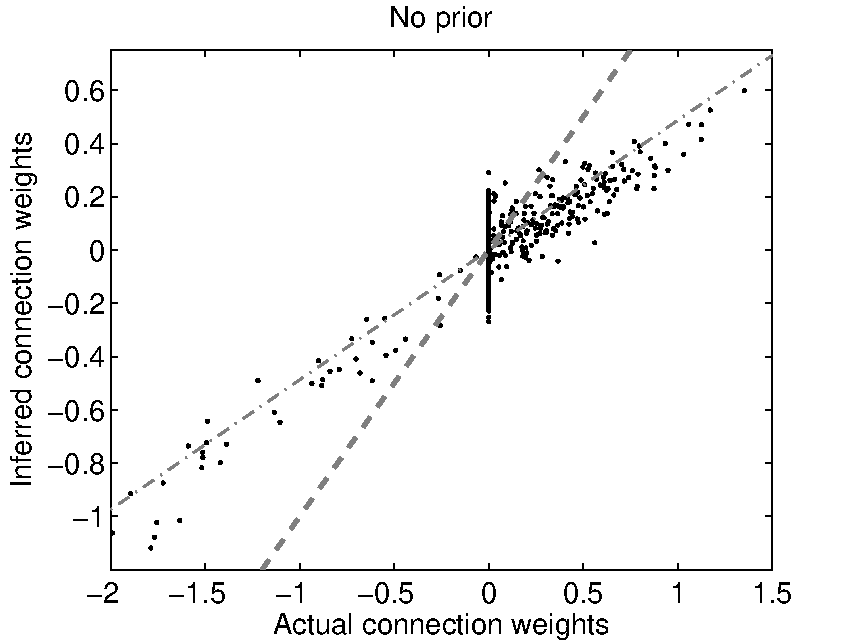
\includegraphics[width=\hsize]{../figs/FigureA10_regular_sol}
\end{minipage}
\begin{minipage}[c]{0.45\hsize}
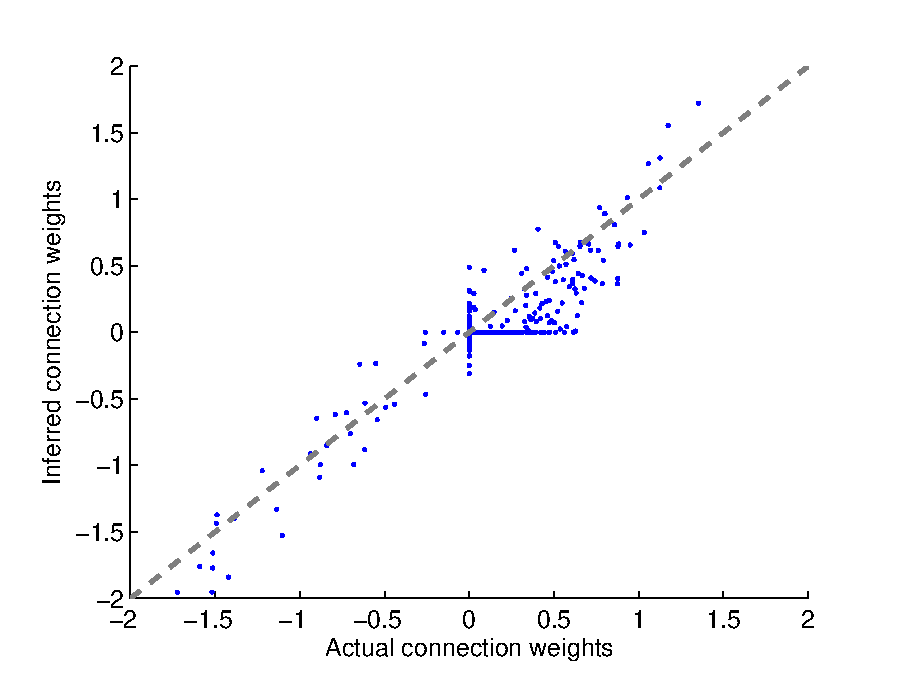
\includegraphics[width=\hsize]{../figs/FigureA10_sparse_sol}
\end{minipage}
\caption{Imposing a sparse prior on connectivity improves our
estimates.  Scatter plots indicate the connection weights $w_{ij}$
reconstructed using no prior ($r^2=0.64$; left panel) and a sparse
prior ($r^2=0.85$; right panel) vs.~the true connection weights in
each case.  These plots were based on a simulation of $N=50$ neurons
firing at $\approx 5$ Hz, imaged for $T=10$ min, with eSNR $\approx
10$.  Clearly, the sparse prior reduces the relative error, as
indicated by comparing the relative distance between the data points
(black dots) to the best linear fit (gray dash-dotted line), at the
expense of some additional soft-threshold bias, as is usual in the
L$_1$ setting.}
\label{fig:sparse}
\end{figure}

\begin{figure}[t!]
\centering
\begin{minipage}[c]{0.45\hsize}
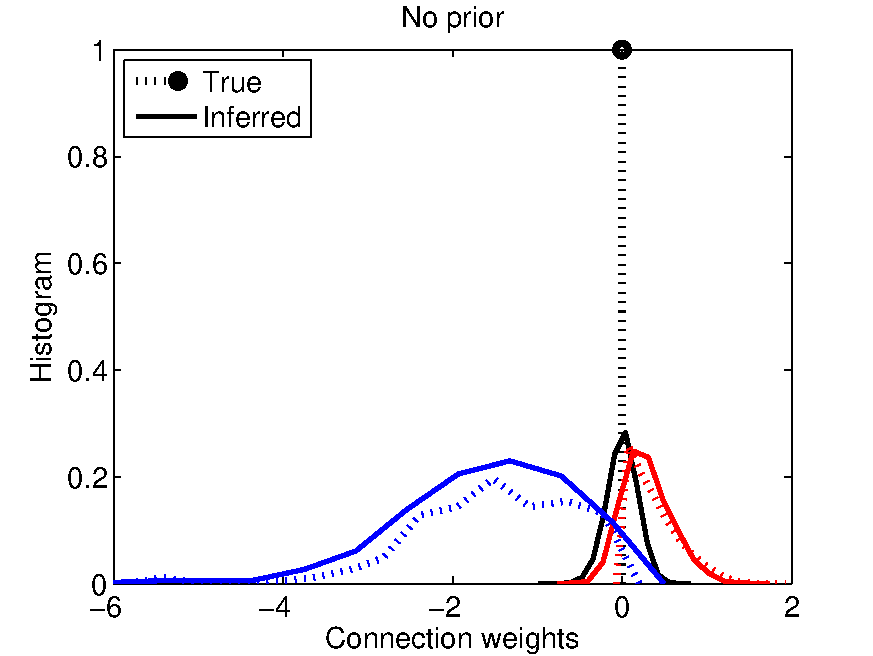
\includegraphics[width=\hsize]{../figs/FigureA3_hist_glm200}
\end{minipage}
\begin{minipage}[c]{0.45\hsize}
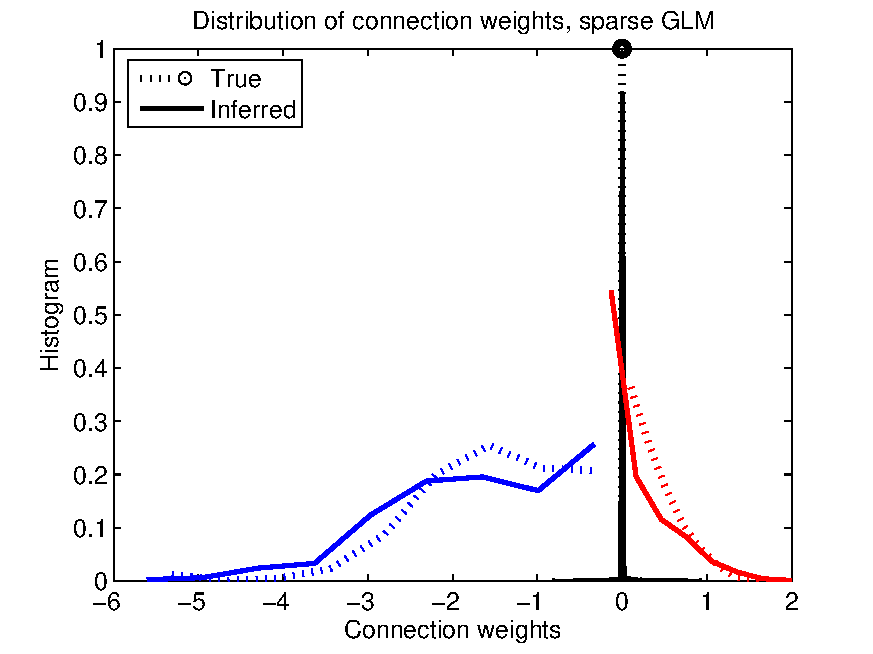
\includegraphics[width=\hsize]{../figs/FigureA3_hist_spa200}
\end{minipage}
\caption{The distributions of inferred connection weights using no
prior (left panel) and a sparse prior (right panel) vs. true
distributions. When the sparse prior is enforced, zero weights are
recovered with substantially higher frequency (black lines), thus
allowing better identification of connected neural pairs. Likewise,
excitatory and inhibitory weights are better recognized (red and blue
lines, respectively), thus allowing accurate classification of neurons
as excitatory or inhibitory. Distributions are shown for a simulated
population of $N=200$ neurons firing at $\approx 5$ Hz and imaged for
$T=10$ min, with eSNR $\approx 10$.  Note that the peak at zero in the
true distributions (black dashed trace) corresponds to the vertical
line visible at zero in Figs.~\ref{fig:scatters} and
\ref{fig:sparse}.}
\label{fig:distros}
\end{figure}


\subsection{Impact of experimental factors on estimator accuracy}

Next we sought to quantify the minimal experimental conditions
necessary for accurate estimation of the connectivity matrix.  Figure
\ref{fig:recvar} shows the quality of the inferred connectivity matrix
as a function of the imaging frame rate, and indicates that imaging
frame rates $\geq 30$ Hz are needed to achieve meaningful
reconstruction results.  This matches nicely with currently-available
technology; as discussed in the introduction, $30$ or $60$ Hz imaging
is already in progress in a number of laboratories
\cite{NguyenParker01,Iyer06,SalomeBourdieu06,ReddySaggau08}, though in
some cases higher imaging rates comes at a cost in the signal-to-noise
ratio of the images or in the number of neurons that may be imaged
simultaneously.


\begin{figure}[t!]
\centering 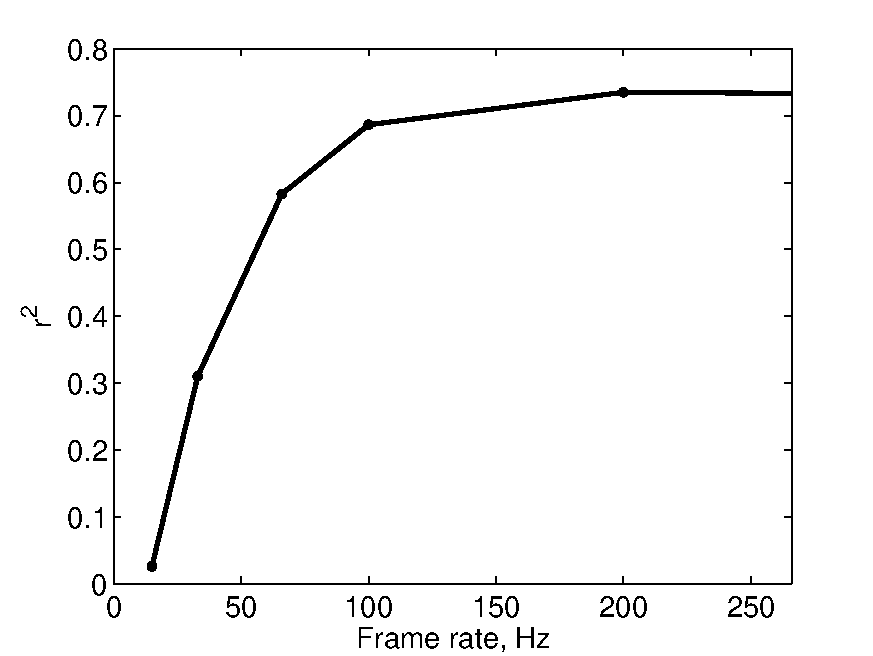
\includegraphics[width=3in]{../figs/FigureA5_recvar}
\caption{Accuracy of the inferred connectivity as a function of the
frame rate of calcium imaging.  A population of $N=25$ neurons firing
at $\approx 5$ Hz and imaged for $T=10$ min was simulated here, with
eSNR $\approx 10$.  At $100$ Hz, $r^2$ saturated at the level
$r^2\approx 0.7$ achieved with $\Delta \rightarrow 0$.}
\label{fig:recvar}
\end{figure}

Similarly, Figure \ref{fig:recvar-SNR} illustrates the quality of the
inferred connectivity matrix as a function of the effective SNR
measure defined in eq.~(\ref{eq:eSNR}); the effective SNR necessary
for accurate reconstructions at these frame rates was $\approx 5$.
Finally, Figure \ref{fig:recvar-NT} shows the quality of the inferred
connectivity matrix as a function of the experimental duration. The
minimal amount of data for a particular $r^2$ depended substantially
on whether the sparse prior was enforced.  In particular, when not
imposing a sparse prior, the calcium imaging duration necessary to
achieve $r^2=0.5$ for the reconstructed connectivity matrix in this
setting was $T\approx 10$ min, and $r^2=0.75$ was achieved at
$T\approx 30$ min.  With a sparse prior, $r^2>0.7$ was achieved
already at $T\approx 5$ min. Furthermore, we observed that the
accuracy of the reconstruction did not deteriorate dramatically with
the size of the imaged neural population: roughly the same
reconstruction quality was observed (given a fixed length of data) for
$N$ varying between $50$--$200$ neurons.  These results were
consistent with a rough Fisher information computation which we
performed but have omitted here to conserve space.


\begin{figure}[t!]
\centering
\begin{minipage}[c]{0.6\hsize}
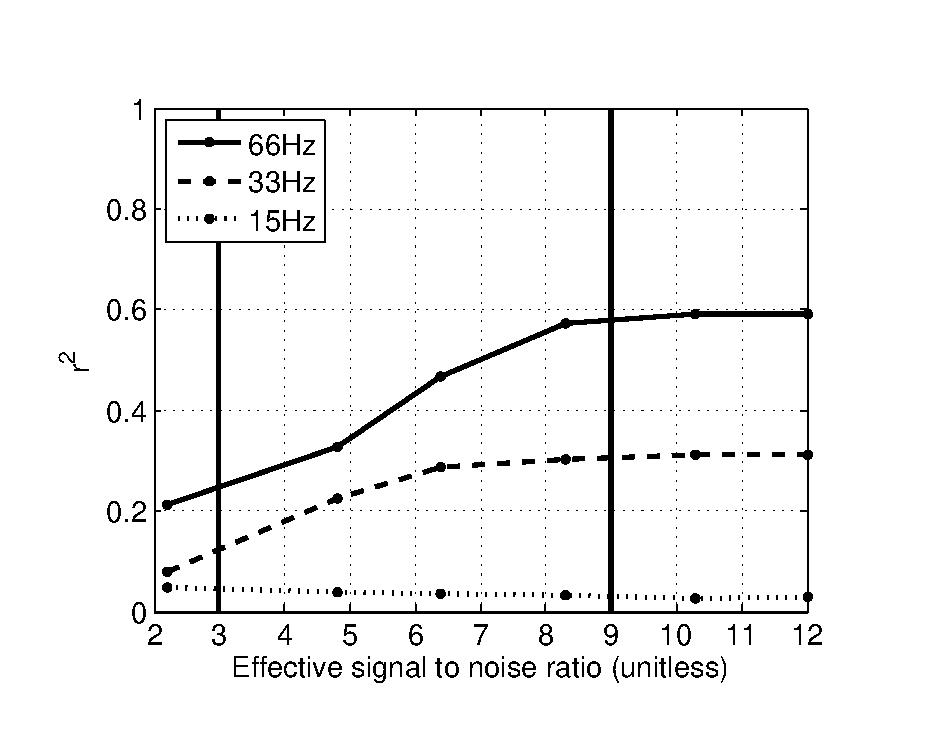
\includegraphics[width=\hsize]{../figs/FigureA6_recvar_SNRc}
\end{minipage}
\caption{Accuracy of inferred connectivity as a function of effective
imaging SNR (eSNR, defined in eq.~\ref{eq:eSNR}), for frame rates of
15, 33, and 66 Hz.  Neural population simulation was the same as in
Figure \ref{fig:recvar}.  Vertical black lines correspond to the eSNR
values of the two example traces in Figure \ref{fig:example_traces},
for comparison.}
\label{fig:recvar-SNR}
\end{figure}


\begin{figure}[t!]
\centering
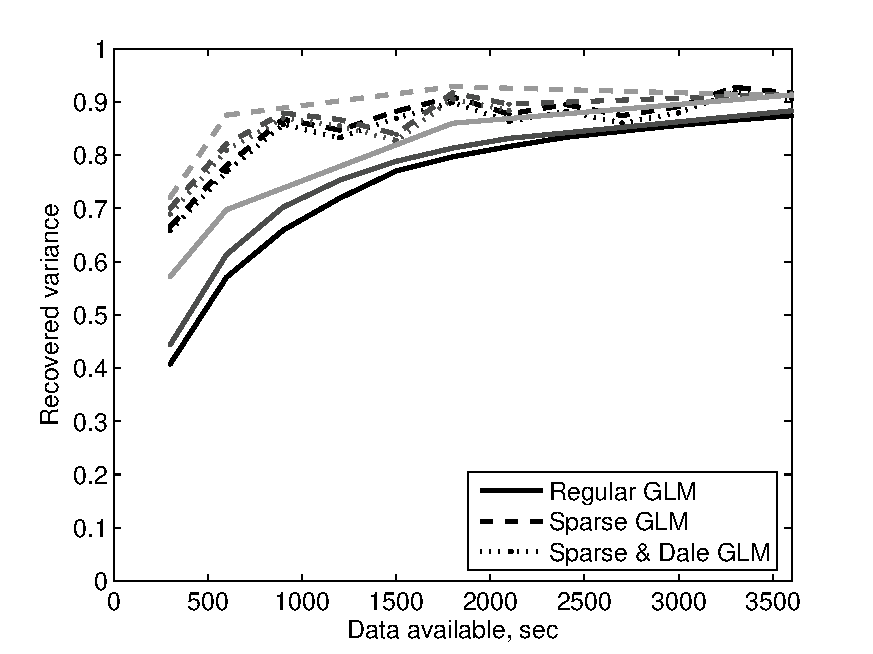
\includegraphics[width=3in]{../figs/FigureA7_recvar_NT}
\caption{Accuracy of inferred connectivity as a function of the
imaging time and neural population size. Incorporating a sparse prior
dramatically increases the reconstruction's quality (dashed
lines). When the sparse prior is imposed, $T=5$ min is already
sufficient to recover $70\%$ of the variance in the connection
weights. Incorporating Dale's prior leads to only marginal improvement
(dotted line). Furthermore, reconstruction accuracy does not strongly
depend on the neural population size, $N$. Here, neural populations of
size $N=10-200$ were simulated for different $T$; $N=100$ and $200$
are shown (black and gray, respectively), with eSNR $\approx 10$ in each
case.}
\label{fig:recvar-NT}
\end{figure}


\comment{

\subsection{Accuracy of the estimates and Fisher information matrix}
\label{sec:methods:accuracy_Fisher} 

Here we calculate theoretically the amount of spike trains data
necessary to accurately estimate the functional connectivity matrix,
$\bw$. For clarity, we assume here that $\Delta \rightarrow 0$, and so
$f(J)\approx e^J\Delta$, and that the spike trains are known
perfectly, i.e. there is no corruption due to inference from low-SNR
calcium imaging data (an assumption validated by the above
results). We also assume that the spikes only couple over a single
time bin, so $h_{ij}(t)\equiv n_j(t-\Delta)$. Then, we can write the
likelihood for the weights:
\begin{align}\label{eqn:fisher-glm}
% \begin{array}{rl}
-\ln P[\bw | \bX] &\propto -\ln P[\bX | \bw] =
\sum\limits_{i,t} \left[ n_i(t) \ln f(J_i(t)) + (1-n_i(t)) (1-f(J_i(t))) \right], \\
J_i(t) &= b_i(t) + \sum\limits_j w_{ij} h_{ij}(t) = b_i(t) + \sum\limits_j w_{ij} n_j(t-\Delta)
%h_{ij}(t) &= n_j(t-\Delta)
.
% \end{array}
\end{align}
The Fisher information matrix for $P[\bw | \bX]$ is therefore:
\begin{multline}\label{eqn:fisher-def}
% \begin{array}{rl}
COV^{-1}_{ij;i'j'}=\left[\frac{\partial (-\ln P[\bw | \bX])}{\partial \w_{ij}\partial \w_{i'j'}}\right]
=\\-\delta_{ii'}\sum\limits_t\left[
n_i(t)n_{j}(t-\Delta)n_{j'}(t-\Delta)\left(-\frac{f'(J_i(t))^2}{f(J_i(t))^2} +
\frac{f''(J_i(t))}{f(J_i(t))}\right) -(1-n_i(t))n_{j}(t-\Delta)n_{j'}(t-\Delta)f''(J_i(t))\right],
% \end{array}
\end{multline}
where $f'$ and $f''$ correspond to the first and the second derivatives of our linking function (c.f Eq.~\eqref{eqn:glm:definition}), and $\delta_{ii'}$ is the Kronecker's delta symbol, i.e., $\delta_{ii'}=1$ for $i=i'$, and $\delta_{ii'}=0$ otherwise.  Letting $f(J)=e^J\Delta$, the first term in the sum in Eq.~\eqref{eqn:fisher-def} cancels out, and the rest may be rewritten as:
\begin{align}\label{eqn:fisher}
% \begin{array}{rl}
COV^{-1}_{ij;i'j'}
&=\delta_{ii'} T P[n_i(t)=0, n_j(t-\Delta)=1, n_{j'}(t-\Delta)=1]% \times \\&
\times E[e^{J_i(t)}|n_i(t)=0, n_j(t-\Delta)=1, n_{j'}(t-\Delta)=1] \nonumber \\
&= \delta_{ii'}T\left[(r \tau^h)\delta_{jj'}+O((r \tau^h)^2)\right]r.
% \end{array}
\end{align}
Here, $TP[n_i(t)=0, n_j(t-\Delta)=1, n_{j'}(t-\Delta)=1]$ describes the number of nonzero
terms in Eq.~\eqref{eqn:fisher-def}, corresponding to the condition that
$(1-n_i(t))n_{j}(t-\Delta)n_{j'}(t-\Delta)$ is only nonzero when
$n_i(t)=0$, $n_j(t-\Delta)=1$, and $n_{j'}(t-\Delta)=1$.  We let $r=E[e^{J_i(t)}|n_i(t)=0, n_j(t-\Delta)=1, n_{j'}(t-\Delta)=1]$  correspond to the average value of $f''(J_i(t))$, conditional on such nonzero events.  $r\tau_h \ll 1$ is the probability for a neuron to spike over the time-interval $\tau_h$.

The Fisher information matrix is block-diagonal, $COV^{-1}_{ij;i'j'} \propto \delta_{ii'}$, due to the structure of the log-likelihood $P[\bX | \bw]$ (it is a sum over $i$ of independent terms), Eq.~\eqref{eqn:fisher-glm}.From Eq.~\eqref{eqn:fisher}, we observe that Fisher information matrix is predominantly diagonal, because $COV^{-1}_{ij;i'j'} \propto \delta_{ii'}\delta_{jj'}$, and thus the covariance matrix, $COV$, can be computed trivially:
\begin{equation}
COV = (rT)^{-1} (r \tau^h I + O((r \tau_h)^2))^{-1} = (r^2 \tau_h T)^{-1} I + O((r \tau_h)^2),
\end{equation}
\noindent where $I$ is the Identity matrix of appropriate size.  For successful determination of the functional connectivity matrix $\bw$, $COV$ should be made smaller than the typical scale $\langle \bw^2\rangle$, so we require that:
\begin{equation}
T \approx (\langle \bw^2 \rangle r^2  \tau^h)^{-1}.
\end{equation}
For typical values of $\langle\bw^2\rangle\approx 0.1$, $r\approx 5$ Hz and $ \tau_h \approx 10$ msec, this estimate provides $T$ of the order of hundreds of seconds. This theoretical estimate of the necessary amount of fluorescent data is in good agreement with our simulations.

Finally, because $COV^{-1}$ is diagonal, this scale of $COV$ does not depend on the number of neurons in the imaged neural population, $N$. Thus, the variance of the estimate $\bw$ does not degrade with the size of the imaged population, $N$, for the same amount of data, $T$.

}


\subsection{Impact of strong correlations and deviations from
  generative model on the inference} 

Estimation of network connectivity is fundamentally rooted in
observing changes in the spike rate conditioned on the state of the
other neurons.  Considered from the point of view of estimating a
standard GLM, it is clear that the inputs to our model
(\ref{eqn:glm:definition}) must satisfy certain basic identifiability
conditions if we are to have any hope of accurately estimating the
parameter $\bw$.  In particular, we must rule out highly
multicollinear inputs $\{h_{ij}(t)\}$: speaking roughly, the set of
observed spike trains ${\bf n}(t)$ should be rich enough to span all
$N$ dimensions of ${\bf w}_i$, for each cell $i$.  In the simulations
pursued here, the coupling matrix $\{w_{ij}\}_{i \neq j}$ was fairly
weak and neurons fired largely independently of each other: see
Fig.~\ref{fig:rasters}, upper left for an illustration.  In this case
of weakly-correlated firing, the inputs $\{h_{ij}(t)\}$ will also be
weakly correlated, and the model should be identifiable, as indeed we
found.  Should this weak-coupling condition be violated, however
(e.g., due to high correlations in the spiking of a few neurons), we
may require much more data to obtain accurate estimates due to
multicollinearity problems.

To explore this issue, we carried out a simulation of a hypothetical
strongly coupled neural network, where in addition to the
physiologically-relevant weak sparse connectivity discussed in section
\ref{sec:results:simulations} we introduced a sparse random strong
connectivity component.  More specifically, we allowed a fraction of
neurons to couple strongly to the other neurons, making these
``command'' neurons which in turn could strongly drive the activity of
the rest of the population \cite{MACLEAN05}.  The strength of this
strong connectivity component was chosen to dynamically build up the
actual firing rate from the baseline rate of $f(b) \approx 1$ Hz to
approximately $5$ Hz. Such a network showed patterns of activity very
different from the weakly coupled networks inspected above (Figure
\ref{fig:rasters}, top right). In particular, a large number of highly
correlated events across many neurons were evident in this network. As
expected, our algorithm was not able to identify the true connectivity
matrix correctly in this scenario (Figure \ref{fig:rasters}, bottom
right panel).  For ease of comparison, the left panels show a
``typical'' network (i.e., one lacking many strongly coupled neurons),
and its associated connectivity inference.

\begin{figure}[t!]
\centering
\begin{minipage}[c]{0.45\hsize}
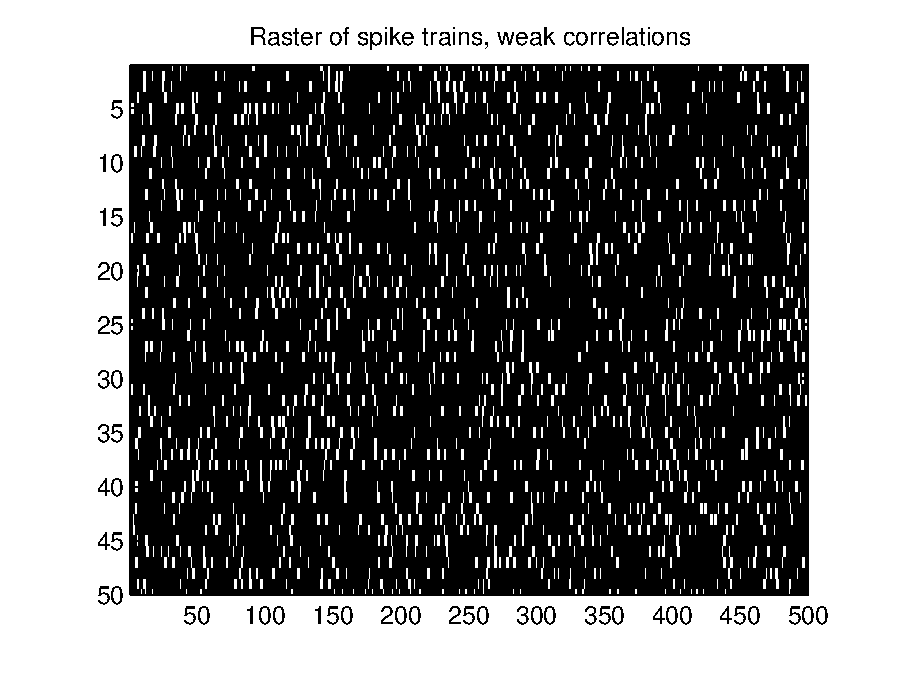
\includegraphics[width=\hsize]{../figs/Figure7b_raster_weak}
\end{minipage}
\begin{minipage}[c]{0.45\hsize}
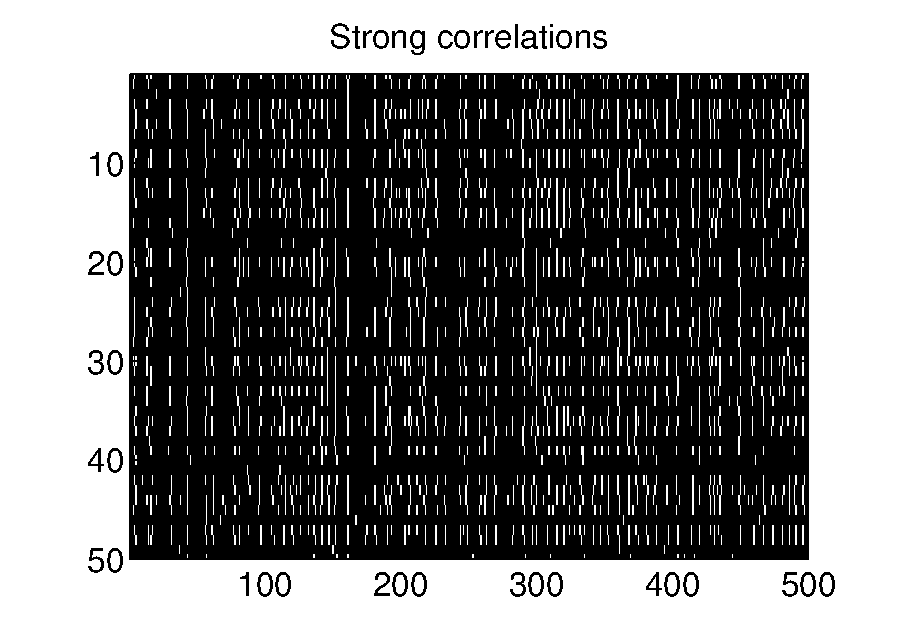
\includegraphics[width=\hsize]{../figs/Figure7a_raster_strong}
\end{minipage}
\begin{minipage}[c]{0.45\hsize}
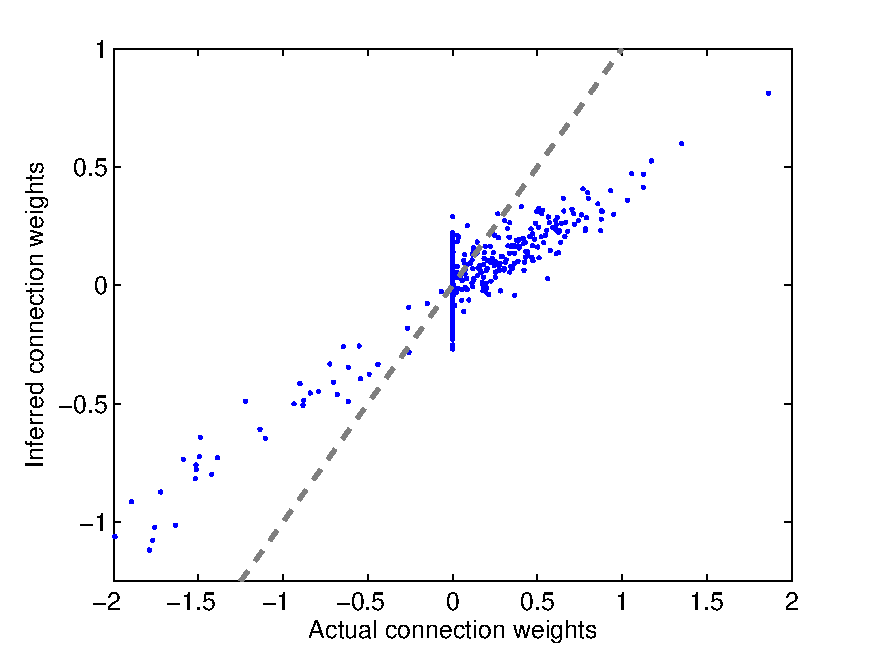
\includegraphics[width=\hsize]{../figs/FigureA8_weak_corr}
\end{minipage}
\begin{minipage}[c]{0.45\hsize}
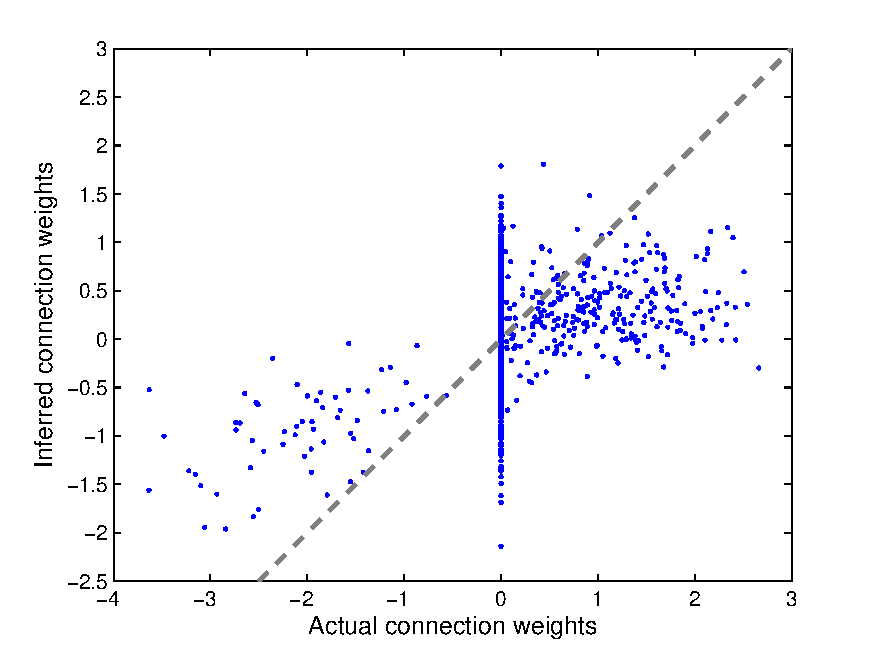
\includegraphics[width=\hsize]{../figs/FigureA8_strong_corr}
\end{minipage}
\caption{Diversity of observed neural activity patterns is required
for accurate circuit inference. Here, 15 sec of
simulated spike trains for a weakly coupled network (top left panel)
and a network with strongly coupled component (top right panel) are
shown. In weakly coupled networks, spikes are sufficiently
uncorrelated to give access to enough different neural activity
patterns to estimate the weights ${\bf w}$. In a strongly coupled
case, many highly synchronous events are evident (top right panel),
thus preventing observation of a sufficiently rich ensemble of activity
patterns. Accordingly, the connectivity estimates for the strongly
coupled neural network (bottom right panel) does not represent the
true connectivity of the circuit, even for the weakly coupled
component. This is contrary to the weakly-coupled network (bottom left
panel) where true connectivity is successfully obtained. Networks of
$N=50$ neurons firing at $\approx 5$ Hz and imaged for $T=10$ min were
used to produce this figure; eSNR $\approx 10$.}
\label{fig:rasters}
\end{figure}

On the other hand, our inference algorithm showed significant
robustness to model misspecifcation, i.e., deviations from our
generative model. One important such deviation, which is likely to
occur in real experiments, is variation in the time scales of PSPs in
different synapses. Up to now, all PSP time-scales were assumed to be
the same in our inference algorithm as well as in the simulations,
i.e., $\{\tau^h_{ij}\}_{i,j\leq N}=\tau_h$. In Figure \ref{fig:vartau}
we introduce additional variability in $\tau_h$ from one neuron to
another. Variability in $\tau_h$ results in added variance in the
estimates of the connectivity weights $w_{ij}$, through the
$\tau_h$-dependence of the scaling factor Eq.~\eqref{eqn:bias}.
However, we found that this additional variance was relatively
insignificant in cases where $\tau_h$ varied up to $25\%$ from neuron
to neuron.

\begin{figure}[t!]
\centering
\begin{minipage}[c]{0.45\hsize}
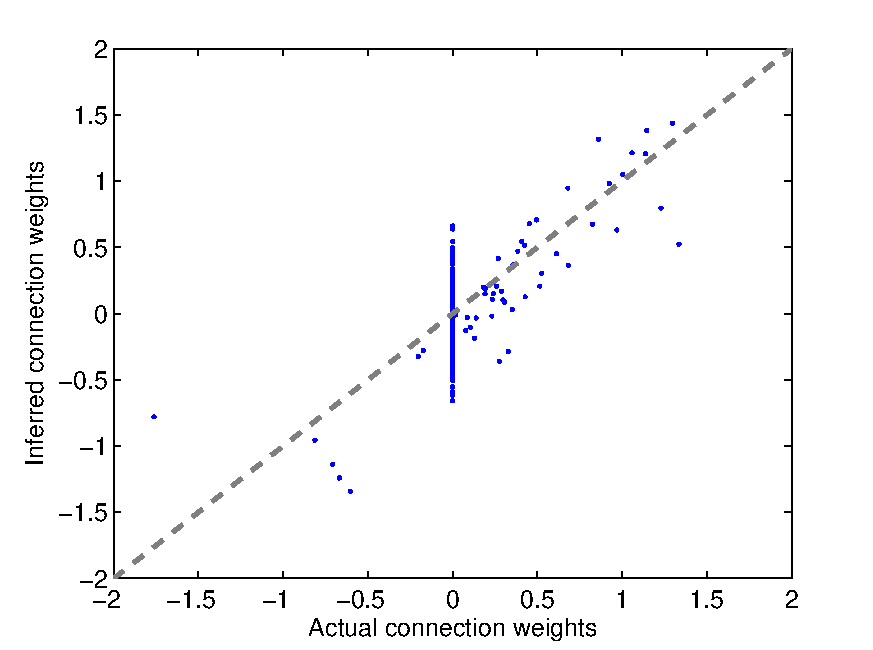
\includegraphics[width=\hsize]{../figs/FigureA9_all_same_sol}
\end{minipage}
\begin{minipage}[c]{0.45\hsize}
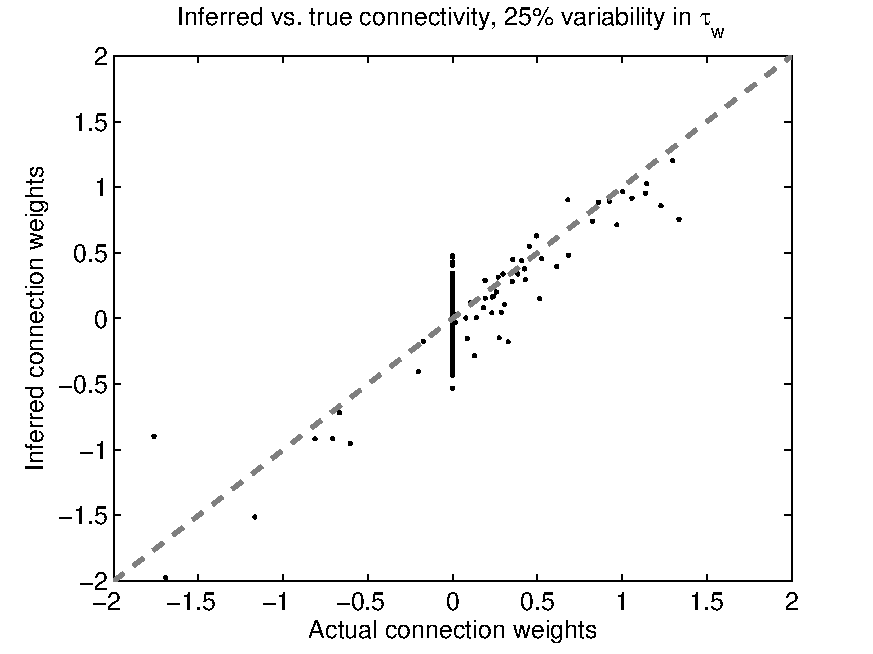
\includegraphics[width=\hsize]{../figs/FigureA9_variable_25}
\end{minipage}
\caption{ Inference is robust to deviations of the data from our
generative model. With up to $25\%$ variability allowed in PSP time
scales $\tau_h$ (right panel), our algorithm provided reconstructions
of almost the same quality as when all $\tau_h$'s were the same (left
panel). Simulation conditions were the same as in Figure
\ref{fig:recvar}.}
\label{fig:vartau}
\end{figure}


\section{Discussion}
\label{sec:discussion}
In this paper we develop a Bayesian approach for inferring
connectivity in a network of spiking neurons observed using calcium
fluorescent imaging.  A number of previous authors have addressed the
problem of inferring neuronal connectivity given a fully-observed set
of spike trains in a network
\cite{BRIL88,CSK88,BRIL92,PAN03d,PAN04c,TRUC05,Rigat06,NYK06,KP06,Vidne08,Stevenson2009,Garofalo09},
but the main challenge in the present work is the indirect nature of
the calcium imaging data, which provides only noisy, low-pass
filtered, temporally sub-sampled observations of spikes of individual
neurons.  To solve this problem, we develop a specialized
blockwise-Gibbs sampler that makes use of an embedded Markov chain
method due to \cite{NBR03}.  The connectivity matrix is then inferred
in an EM framework; the M-step parallelizes quite efficiently and
allows for the easy incorporation of prior sparseness information,
which significantly reduces data requirements in this context.  We
have found that these methods can effectively infer the connectivity
in simulated neuronal networks, given reasonable lengths of data,
computation time, and assumptions on the biophysical network
parameters.

To our knowledge, we are the first address this problem using the
statistical deconvolution methods and EM formulation described here
(though see also \cite{Roxin08}, who fit simplified, low temporal
resolution transition-based models to the 10 Hz calcium data obtained
by \cite{IkegayaYuste04}).  However, we should note that
\cite{Rigat06} developed a closely related approach to infer
connectivity from low-SNR electrical recordings involving
possibly-misclassified spikes (in contrast to the slow,
lowpass-filtered calcium signals we discuss here).  In particular,
these authors employed a very similar Bernoulli GLM and developed a
Metropolis-within-Gibbs sampler to approximate the necessary
sufficient statistics for their model.  In addition, \cite{Rigat06}
develop a more intricate hierarchical prior for the connectivity
parameter $\bw$; while we found that a simple L$_1$ penalization was
quite effective here, it will be worthwhile to explore more
informative priors in future work.

A number of possible improvements of our method are available.  One of
the biggest challenges for inferring neural connectivity from
functional data is the presence of so called hidden inputs from
unobserved neurons \cite{Nykamp05,NYK06,KP06,Vidne08,Vakorin09}.  It
is typically impossible to observe the activity of all neurons in a
given circuit, and correlations in the unobserved (``hidden'') inputs
can mimic functional connections among different observed neurons,
thus presenting a substantial challenge for estimating neural
connectivity.  Developing methods to cope with such hidden inputs is
currently an area of active research, and should certainly be
incorporated in the methods we have developed here.

Several other important directions for future work are worth noting.
First, recently-developed photo-stimulation methods for activating or
deactivating individual neurons or sub-populations
\cite{Deisseroth05,SzobotaIsacoff07,Nikolenko08} may be useful to
increase statistical power in cases where the circuit's unperturbed
activity may not allow reliable determination of a circuit's
connectivity matrix; in particular, by utilizing external stimulation,
we can in principle choose a sufficiently rich experimental design
(i.e., a sample of input activity patterns) to overcome the
multicollinearity problems discussed in the context of
Fig.~\ref{fig:rasters}.

Second, improvements of the algorithms for faster implementation are
under development.  Specifically, fast non-negative optimization-based
deconvolution methods may be a promising alternative
\cite{Vogelstein08,Pan08b} to the SMC approach used here.  In
addition, modifications of our generative model to incorporate
non-stationarities in the fluorescent signal (e.g., due to dye
bleaching and drift) are fairly straightforward.

Third, a fully Bayesian algorithm for estimating the posterior
distributions of all the parameters (instead of just the MAP estimate)
would be of significant interest.  Such a fully-Bayesian extension is
conceptually simple: we just need to extend our Gibbs sampler to
additionally sample from the parameter $\bth$ given the sampled spike
trains $\bX$. Since we already have a method for drawing $\bX$ given
$\bth$ and $\bF$, with such an additional sampler we may obtain
samples from $P(\bX,\bth | \bF)$ simply by sampling from $\bX \sim
P(\bX|\theta,\bF)$ and $\bth \sim P(\bth |\bX)$, via blockwise-Gibbs.
Sampling from the posteriors $P(\bth|\bX)$ in the GLM setting is quite
tractable using hybrid Monte Carlo methods, since all of the necessary
posteriors are log-concave
\cite{Ishwaran99,Gamerman97,Gamerman98,Yashar08}.

Finally, most importantly, we are currently applying these algorithms
in preliminary experiments on real data.  Checking the accuracy of our
estimates is of course more challenging in the context of
non-simulated data, but a number of methods for partial validation are
available, including multiple-patch recordings \cite{Song2005},
photostimulation techniques \cite{Vovan07}, and fluorescent anatomical
markers which can distinguish between different cell types
\cite{Meyer02} (i.e., inhibitory vs.\ excitatory cells; c.f.\
Fig.~\ref{fig:distros}).  We hope to present our results in the near
future.

% \begin{acknowledgments}
\section*{Acknowledgements}
The authors would like to acknowledge R.\ Yuste, B.\ Watson, A.\
Packer, T.\ Sippy, T.\ Mrsic-Flogel, and V.\ Bonin for data and
helpful discussions, and A.\ Ramirez for helpful comments on an
earlier draft.  LP is supported by an NSF CAREER and McKnight Scholar
award; JV by NIDCD grant DC00109.
% \end{acknowledgments}

\bibliography{mybib}
% \bibliographystyle{amsplain}
\bibliographystyle{apalike}

\end{document}
